%%%%%%%%%%%%%%%%%%%%%%%%%%%%%%%%%%%%%%%%%%%%%%
% To select a journal, use its code for the 
% journal= option in the \documentclass command.
% The journal codes for this template are:

% Wearable Technologies: wet
% Data and Policy: dap
% Data-centric Engineering: dce
% Environmental Data Science: eds
% Programmable Materials: prm
% Journal of Nonlinear Waves: jnw
% Flow: flw
% Judgment and Decision Making: jdm
% Psychometrika: psy
% Forum of Mathematics, Pi: fmp
% Forum of Mathematics, Sigma: fms
% Glasgow Mathematical Journal: gmj
% Research Synthesis Methods: rsm
%%%%%%%%%%%%%%%%%%%%%%%%%%%%%%%%%%%%%%%%%%%%%%
\documentclass[journal=rsm]{CUP-JNL-DTM}%


% If using any of the following journal options:
%   wet, dap, dce, eds, prm, jnw, flw, jdm, psy, rsm
% then uncomment the following line:
\addbibresource{reference_update.bib}
\AtEveryBibitem{%
  \clearfield{note}%
  \clearfield{keywords}%
  \clearfield{abstract}%
  \clearfield{issn}%
  \clearfield{eprint}%
  \ifentrytype{article}{\clearfield{url}}{}%
}


%%%% Packages
\usepackage{graphicx}
\usepackage{multicol}
\usepackage{amsmath,amssymb,amsfonts}
\usepackage{amsthm}
\usepackage[T1]{fontenc}
\usepackage{newtxtext}
\usepackage{newtxmath}
\usepackage{textcomp}
\usepackage{xcolor}
\usepackage[colorlinks,allcolors=blue]{hyperref}
%%%%


%%%% Additional packages required by the manuscript content
\usepackage{placeins}
\graphicspath{ {./images/} }
%%%%


\newtheorem{theorem}{Theorem}[section]
\newtheorem{lemma}[theorem]{Lemma}
\theoremstyle{definition}
\newtheorem{remark}[theorem]{Remark}
\newtheorem{example}[theorem]{Example}
\numberwithin{equation}{section}


\jname{Research Synthesis Methods (RSM)}
\articletype{Research Articles}
%\artid{20}
\jyear{2026}
%\jvol{4}
%\jissue{1}
%\raggedbottom


\begin{document}

\begin{Frontmatter}

\title[Meta-Analysis for Heterogeneous Exposure Intervals]
{Contrast-Level Aggregate-Data Dose--Response\protect\\
Meta-Analysis for Heterogeneous Exposure Intervals}

% There is no need to include ORCID IDs in your .pdf; this information is captured by the submission portal when a manuscript is submitted. 
\author[1]{Yangyifan Lu}
\author*[1,2]{Chong Wang}
\author[3]{Brayan Alexander Fonseca Martinez}
\author[4]{Jan M. Sargeant}
\author[5]{Sarah C. Totton}
\author[3]{Annette M. O'Connor}

\authormark{Yangyifan Lu \textit{et al}.}

\address[1]{\orgdiv{Department of Statistics}, \orgname{Iowa State University}, \orgaddress{\city{Ames}, \postcode{50011}, \state{IA},  \country{USA}}. \email{ylu1@iastate.edu}}

\address*[2]{\orgdiv{Department of Veterinary Diagnostic and Production Animal Medicine}, \orgname{Iowa State University}, \orgaddress{\city{Ames}, \postcode{50011}, \state{IA},  \country{USA}}. \email{chwang@iastate.edu}}

\address[3]{\orgdiv{Department of Large Animal Clinical Sciences}, \orgname{Michigan State University}, \orgaddress{\city{East Lansing}, \postcode{48824}, \state{MI},  \country{USA}}. \email{bafonseca258@gmail.com; oconn445@msu.edu}}

\address[4]{\orgname{Independent Contractor}, \orgaddress{\city{Guelph}, \state{ON},  \country{Canada}}. \email{sargeanj@uoguelph.ca}}

\address[5]{\orgdiv{Independent Contractor}, \orgname{Ontario Veterinary College, University of Guelph}, \orgaddress{\city{Guelph}, \postcode{N1G 2W1}, \state{ON},  \country{Canada}}. \email{sarah.totton@gmail.com}}

\keywords{contrast-level aggregate-data meta-analysis, dose--response meta-analysis, heterogeneous exposure supports, interval exposure, exact exposure values, random-effects meta-regression}

\abstract{Meta-analysis is complicated when studies report adjusted odds ratios for study-specific pairs of exposure or intervention intervals but individual data, group frequencies, and outcome counts are unavailable. We propose a support-based contrast-level aggregate-data dose--response meta-analysis method for interval and exact supports. An outcome-independent support-to-design operator maps each comparison and reference support to the expected dose--response basis under a working exposure distribution. With the implemented linear basis, this is the support-specific mean; an exact value is a zero-width interval mapped to itself. Differences between the mapped supports are used as design covariates in a contrast-level working mixed model fitted by generalized least squares or profile restricted maximum likelihood. The approach retains arbitrary support pairs without recoding them to a common reference interval. Conventional point-dose and midpoint dose--response meta-analysis are exact special cases.

Under a correctly specified Gamma working distribution, slope bias was less than 0.001 in the empirical mixed-support simulation; severe distributional misspecification produced bias of $-0.290$. In the principal 16-study residential-radon illustration, a historical country-specific Lognormal mapping gave an odds ratio of 1.081 per 100 Bq/m$^3$ (95\% confidence interval 1.032--1.133), with sensitivity to the assumed within-study correlation. A motivating eight-study animal-feeding-operation working analysis combines explicit-distance odds ratios and proxy mappings, with OR-only and explicit-support restriction analyses. Published randomized-trial meta-analyses provide examples of the same support-representation problem. The method is appropriate when the working exposure distribution is defensible; otherwise sensitivity analysis is essential.}

\end{Frontmatter}

\newpage
\section*{Highlights}

\noindent\textbf{What is already known}
\par
Conventional dose--response meta-analysis generally assigns a single exposure value to each reported exposure category. Existing methods for grouped exposures often require individual participant data or group-level exposure--outcome information that may not be available in published studies.

\noindent\textbf{What is new}
\par
We introduce a support-to-design operator for contrast-level aggregate data when published studies provide pairwise adjusted odds ratios and their uncertainty but the comparison and reference exposures are heterogeneous intervals or exact points. The operator maps each support to a distribution-dependent average dose--response basis vector before standard meta-regression. It requires neither exposure-group frequencies nor outcome counts, retains arbitrary reported support pairs, and contains conventional point-dose and midpoint dose--response meta-analysis as exact special cases.

\noindent\textbf{Potential impact for Research Synthesis Methods readers}
\par
The method permits dose--response synthesis when comparison and reference
intervals differ across studies and only reported contrasts and their
uncertainty measures are available. It also accommodates mixtures of positive-
and zero-width intervals and makes the working exposure-distribution assumption
explicit. It therefore replaces an otherwise analyst-chosen point score with
an auditable support model rather than eliminating the need for a within-support
assumption. The support problem can arise in observational exposure studies and
in randomized trials that assign intervention target ranges.

% \section*{Impact Statement}
% Some Data journals (DAP, DCE) require an `Impact Statement' section. Comment out this section if it is not required.


\section{Introduction}\label{sec1}

Synthesizing research results from multiple studies is essential for
understanding patterns of risk and informing policy. The use of meta-analysis
for the quantitative synthesis of randomized controlled trials (RCTs) and
observational studies is well established. A recurring difficulty arises when
continuous exposure or intervention levels are reported through heterogeneous
intervals rather than common point values. This problem is often encountered in
observational research. When assessing unintended and unplanned exposures that
may cause disease, observational studies are often necessary for ethical and
practical reasons. Because such exposures are not deliberately assigned or
standardized, the exposure definitions and effect measures reported by
observational studies may vary considerably, making quantitative synthesis
difficult. An example of this
problem in environmental health is the association between exposure to
emissions from large animal production facilities and the health of residents
in surrounding communities
~\cite{OConnor_A_M2010,OConnor_A_M2017}. This topic has been of interest
to public health and environmental researchers for many years and has generated
a body of evidence with disparate exposure measures, outcomes, and effect
measures. This variation has made quantitative synthesis difficult. In this
study, we address several of the challenges involved in synthesizing this body
of evidence.

Conventional dose--response meta-analysis (DRMA) based on contrast-level
aggregate data generally requires each exposure category to be represented by a single
quantitative exposure value before a dose--response trend can be estimated
~\cite{Greenland1992,Orsini2012}. A practical difficulty arises when studies
report exposure through intervals with different boundaries and only the resulting reported association estimates and confidence intervals
are available.
In this setting, the original individual-level exposures, exposure-group
counts, and observed mean exposures within the reported categories may be
unavailable.

Related methods have addressed grouped or interval-censored exposures, but
they require information that is not typically available when a
meta-analysis is based on published effect estimates. Cook et
al.~\cite{Cook2001} developed a retrospective likelihood approach using the
joint information on exposure categories and disease status. That likelihood
cannot be constructed when the primary studies report only odds ratios and
confidence intervals without the underlying individual-level data or grouped
exposure--outcome counts.

Allen et al.~\cite{Allen2020,Allen2020b} proposed estimating the mean exposure
within reported intervals as a dose pre-analysis step. Their procedure uses
the interval boundaries together with the numbers or proportions of
individuals in the exposure groups to estimate the exposure distribution. It
then uses reconstructed effective counts in a Bayesian dose--response
likelihood. Such exposure-group frequencies are not consistently available in
the studies included in the present review. Moreover, their grouped-data
likelihood is not applicable to reported adjusted relative association
estimates comparing different pairs of exposure intervals. Their applied
pipeline is useful when those richer grouped data are available, but it is not
applicable when the input consists only of adjusted relative association
estimates, confidence intervals, and support bounds. Calculation of a
conditional group mean is therefore not itself claimed as new here. Our
contribution is a general support-level dose--response model, its formal
properties, and inference for contrast-level summary data without group
frequencies or exposure--outcome counts.

Takahashi and Tango~\cite{Takahashi2010} considered the assignment of
representative exposure values when summarized response data are available
for grouped exposure categories. Their likelihood requires
category-specific response information that is not recoverable from reported
odds ratios and confidence intervals alone.

Shi and Copas~\cite{ShiCopas2004} modeled arbitrarily aggregated dose levels,
and Hartemink et al.~\cite{Hartemink2006} addressed differing exposure
cutpoints and nonlinear dose--response functions. Both are important close
precedents, but their formulations use category-level structures and ordinarily
a study reference category rather than arbitrary pairs of published adjusted
contrasts. Riley et al.~\cite{Riley2015} developed multivariate meta-analysis
for prognostic effects reported at multiple cutpoints, including within-study
dependence and functional trends across cutpoints. That framework synthesizes
cutpoint-specific prognostic effects rather than mapping arbitrary pairs of
exposure supports to representative exposure contrasts. Yu et al.~\cite{Yu2013} compared conventional one- and two-stage
summarized-data DRMA using all reported categories. Most recently, Bauleo et
al.~\cite{Bauleo2026} proposed a categorical-to-continuous conversion based on
category midpoints, category-specific continuous coefficients, and independence
of those estimates. That practical procedure therefore retains the midpoint
and covariance assumptions examined here.

The present review therefore has a different and common contrast-level
aggregate-data structure. Here, contrast-level aggregate data refer to
reported adjusted OR estimates and confidence intervals for comparisons between
exposure groups, in contrast to group-level aggregate data such as event
counts and denominators within each exposure interval. Each available observation is a reported adjusted OR estimate comparing a
study-specific pair of exposure intervals, while the underlying individual participant data and group-level aggregate data are unavailable. The comparison and reference
intervals may differ across observations, and multiple observations from the
same study may involve overlapping or nested intervals. Exact exposure values
are represented as intervals of width zero. Consequently, no method we identified is applicable to
the complete combination of reported inputs in this meta-analysis: adjusted
contrasts whose comparison and reference supports vary by observation,
mixtures of intervals and exact values, within-study dependence, and no
exposure-group frequencies or exposure--outcome counts. The close methods
above remain complementary when their richer or more restrictive input
structures are available.

Conventional summarized-data dose--response meta-analysis becomes operable
only after the analyst supplies a point score for every support, while
retrospective and dose pre-analysis methods require grouped exposure
frequencies or exposure--outcome information that is missing here.
The unresolved problem is therefore not the absence of a downstream
meta-regression estimator, but the absence of a principled mapping from each
reported pair of heterogeneous supports to the quantitative contrast required
by that estimator. We formalize that mapping as the support-to-design operator
\begin{equation}
 \mathcal M_{F_k,h}(S)=E_{F_k}\{h(D)\mid D\in S\},
 \qquad
 X_{kj}=\mathcal M_{F_k,h}(A_{kj})-
         \mathcal M_{F_k,h}(B_{kj}),
 \label{eq:support_operator_intro}
\end{equation}
Here, $D$ is the continuous exposure, $F_k$ is the working exposure
distribution for study $k$, $h$ is the selected dose--response basis, $S$ is
an exposure support, and $A_{kj}$ and $B_{kj}$ are the comparison and reference
supports for observation $j$ in study $k$.
The operator separates outcome-independent support harmonization from conventional
second-stage synthesis. This also separates \emph{support uncertainty} in the
first-stage mapping from \emph{synthesis uncertainty} conditional on that
mapping.

The same support-representation problem also occurs in randomized trials, which may
assign participants to target ranges rather than exact doses, leaving the same
support-representation problem when a meta-analysis uses published treatment
contrasts. Two published examples motivate this broader application. Zhou et
al.~\cite{Jing2012} synthesized 24 randomized trials involving 10,361 patients
with chronic kidney disease whose higher and lower hemoglobin target supports
varied across trials. Cumpstey et al.~\cite{Cumpstey2022} synthesized eight
randomized trials involving 4,415 mechanically ventilated patients and
explicitly identified heterogeneous and overlapping oxygen target ranges.
These examples show that interval-valued supports also arise in clinical-trial
meta-analysis; implementation of the proposed dose--response model requires
variation in the target contrasts and a justified working distribution within
each target range.

Our approach addresses this setting by representing each comparison and
reference interval by the mean exposure within that interval under a
specified working exposure distribution. An exact value is represented as a zero-width interval whose representative mean is the point itself. Their difference defines the
quantitative exposure contrast associated with the reported log odds ratio,
and the resulting contrasts are synthesized using a random-effects
meta-regression.

We obtained data from an ongoing living systematic review that builds on two
previously published systematic reviews of associations between residential
exposure to animal feeding operations and human health
~\cite{OConnor_A_M2010,OConnor_A_M2017,Martinez2026,FonsecaMartinezDAG2026}. The studies identified by the review reported five major categories of health outcomes: lower respiratory diseases, upper respiratory diseases, antimicrobial resistance, infectious conditions, and gastrointestinal diseases.

The present analysis focused on lower respiratory disease (LRD) outcomes and
distance-based measures of residential proximity to the nearest animal feeding
operation (AFO), because these formed the largest subset of evidence that could
be represented using distance intervals. Across studies, residential proximity
was reported using heterogeneous categories and threshold-based contrasts,
creating a need for a method that maps the reported comparisons onto a common
distance scale.

Our objective was to develop and evaluate a contrast-level aggregate-data dose--response meta-analysis method for heterogeneous exposure intervals. The method represents each reported positive-width exposure interval by its mean exposure
under a specified working exposure distribution, while an exact exposure value is represented by the point itself. The difference between the
mean exposures in the comparison and reference supports defines a
quantitative exposure contrast that can be incorporated directly into a
random-effects meta-regression of the reported log odds-ratio estimates.

The proposed model is analogous to a conventional fixed-dose
dose--response model: the difference between two fixed exposure values is
replaced by the difference between the mean exposures within two reported
intervals. When every support
has width zero, this replacement is the identity and the proposed model is
exactly the conventional point-dose model. It therefore inherits the usual
linear or nonlinear dose--response basis, fixed- or random-effects structure,
GLS or REML estimation, covariance modeling, and diagnostics in that special
case. It accommodates heterogeneous interval boundaries and reference groups
without requiring individual participant data or group-level aggregate data, and without recoding all comparisons to a common reference category. The generalized support family additionally includes exact points. The usual midpoint assignment is recovered as a special case when exposure is uniformly distributed within a bounded interval. Although motivated by residential distance, the same contrast-level
aggregate-data structure can arise for other continuous exposures reported
through study-specific intervals.


\section{Method} \label{sec2}

\subsection{Contrast-level aggregate-data structure with heterogeneous exposure intervals}
\label{sec:data_structure}

We consider a set of $K$ studies, indexed by $k=1,\dots,K$, where
study $k$ reports $n_k$ adjusted log odds ratio (log OR) estimates comparing
outcomes between exposure-defined groups. The number of comparisons may vary
across studies, reflecting differences in exposure categorization and study
design. Let $y_{kj}=\log OR_{kj}$ denote this observed estimate for comparison
$j$ in study $k$. The statistical development below is formulated for log
ORs. Any use of another reported measure as an approximate OR is an
application-specific working assumption that must be justified and examined
in sensitivity analysis.

Let $A_{kj}$ and $B_{kj}$ denote the comparison and reference exposure
intervals, respectively, for observation $j$ in study $k$. The corresponding
contrast-level aggregate-data observation is the reported adjusted log OR for
this support pair,
\[
  y_{kj}=\log\widehat{\mathrm{OR}}^{\mathrm{adj}}_{kj}(A_{kj}:B_{kj}).
\]
The study-specific covariate adjustment or standardization is part of the
reported estimand and cannot be reconstructed from contrast-level aggregate
data alone.

The comparison and reference intervals may differ across observations and
across studies. Multiple observations from the same study may also involve
overlapping or nested intervals rather than a common set of mutually
exclusive exposure categories.

All practical supports are represented by the unified interval notation
\begin{equation}
  \mathcal I(a,b)=
  \begin{cases}
    (a,b], & a<b,\\
    \{a\}=[a,a], & a=b,
  \end{cases}
  \qquad 0\leq a\leq b<\infty.
  \label{eq:support_family}
\end{equation}
Thus, an exact exposure value is the special case of an interval with width
zero. In practice, even a category reported as $D>d$ arises from a study
population with finite operational exposure support and can be represented as
$(d,d_{\max}]$, where $d_{\max}$ is the study-specific maximum distance used
to delimit that population. This was the convention used in the empirical
illustration. A genuinely right-unbounded support $(d,\infty)$ is also
accommodated as a theoretical special case, as described below.
 
Each reported OR is accompanied by a 95\% confidence interval. Under standard large-sample approximations, the log OR is approximately normally distributed~\cite{Greenland1992, Orsini2012}. The corresponding standard error is recovered from the reported confidence limits as:

%

\begin{equation}
  \hat{\sigma}_{kj}
    = \frac{\log(UL_{kj}) - \log(LL_{kj})}{2 \times 1.96},
  \label{eq:se}
\end{equation}

%

and is used as the estimated sampling standard deviation of the observed log OR under the normal approximation. Here, $UL_{kj}$ and $LL_{kj}$ denote the upper and lower bounds of the reported 95\% confidence interval for comparison $j$ in study $k$. These standard errors define the diagonal elements of the within-study covariance matrix $\boldsymbol{\Sigma}_k$.

Thus, the required aggregate data for each observation are the reported
effect estimate, its standard error or confidence interval, and the
boundaries of the comparison and reference exposure intervals. For a
zero-width interval, the coincident lower and upper boundaries identify the
exact point value. The method
additionally requires a working exposure distribution from which the mean
exposure within each positive-width interval can be calculated. Individual participant
data, exposure-group frequencies, and grouped exposure--outcome counts are
not required.

The exposure distribution is a first-stage, outcome-independent component of
the analysis and is not nonparametrically identified by the reported relative
association estimates alone without additional restrictions on both the
exposure family and the outcome model. We therefore recommend the following hierarchy. First, use a
reported empirical group mean, or a study-population exposure distribution,
when either is available. Second, when only exposure-interval frequencies are
reported, fit a scientifically plausible distribution by the corresponding
grouped-data likelihood and calculate its conditional means; a Lognormal model
for multiplicative environmental exposures is one example~\cite{Allen2020}.
Third, use a population-relevant external distribution, with explicit
justification and sensitivity analysis. When none of these sources is
available, midpoint assignment remains an identifiable Uniform working-model
special case, but it should be labeled as such and accompanied by sensitivity
analyses over plausible skewed distributions and support bounds. Distribution
selection should not use the outcome contrasts, because doing so would make the
exposure scores outcome-adaptive. If several families remain plausible, the
meta-analysis can be repeated across them or the support means can be averaged
using prespecified first-stage model weights. Uncertainty from an estimated
first-stage distribution can be propagated as described in
Section~\ref{sec:support_uncertainty}.

\noindent\textbf{Practical algorithm.}
For application, the support-to-design procedure has five steps:
\begin{enumerate}
\item retain each adjusted log OR, its standard error, study identifier, and
the reported comparison and reference supports;
\item select an outcome-independent exposure distribution using the hierarchy
above and record the evidence supporting that choice;
\item calculate the conditional mean of every positive-width support and use
the reported value for every zero-width support;
\item subtract the reference mean from the comparison mean for each contrast
and fit the GLS or profile-REML model, preserving within-study blocks; and
\item report sensitivity to plausible exposure distributions, support bounds,
working correlations, and finite-study inference. If no distribution can be
supported, report midpoint scoring explicitly as a Uniform working-model
analysis rather than as an observed mean.
\end{enumerate}

\noindent\textbf{Worked support-to-design example.}
In the radon illustration, Blot et al.'s adjusted OR of $0.90$ compares
$74$--$147$ Bq/m$^3$ with the reported reference support below $74$ Bq/m$^3$.
Under the prespecified Chinese Lognormal distribution (geometric mean 20,
geometric standard deviation 2.2), the representative-mean definition in
Equation~\ref{eq:unified_mean} gives
conditional means $96.47$ and $23.18$ Bq/m$^3$. The resulting design value is
$x=96.47-23.18=73.30$ Bq/m$^3$, and the response supplied to the second-stage
model is $y=\log(0.90)=-0.105$. This calculation is repeated row by row; an
exact exposure would enter directly as its reported point value. The
analysis-ready workbook records the reported bounds, distribution parameters,
conditional means, and design contrasts so the complete mapping is auditable.

The observed log ORs reported within the same study are likely to be
correlated because they are derived from the same underlying study population
and may involve overlapping exposure groups. For example, a study may report
one comparison between $(0,3]$ and $(3,d_{\max}]$ and another between
$(0,6]$ and $(6,d_{\max}]$. Residents contributing to the first comparison
may therefore also contribute to groups in the second comparison, inducing
dependence among the reported estimates. Standard dose--response and
multivariate meta-analysis methods account for such dependence through the
within-study covariance structure~\cite{Greenland1992, Orsini2012}. However,
the studies included in our analysis generally reported only odds ratios and
confidence intervals, without sufficient information to reconstruct the full
covariance matrix.

Therefore, we estimated the marginal variances of the log ORs using the reported confidence limits (Equation~\ref{eq:se}) and approximated the within-study covariance structure by assuming a common correlation parameter $\rho$ across comparisons within the same study~\cite{Higgins1996}. The use of plausible working correlation assumptions when the within-study covariance structure is unavailable has been discussed in the multivariate meta-analysis literature~\cite{Jackson2011, Wei2012}. This treats multiple estimates from a study in the same aggregate-data manner commonly used in multivariate meta-analysis when the exact covariance matrix is unavailable. In the meta-analysis, we used $\rho = 0.5$ as the working correlation assumption and further evaluated the sensitivity of the results under alternative values of $\rho$.

Collecting all $n_k$ log ORs within study $k$ into a vector $\mathbf{y}_k$, the joint within-study distribution is specified as:

%

\begin{equation}
\mathbf{y}_k \sim \mathrm{MVN}\!\left(
    \boldsymbol{\eta}_k,\; \boldsymbol{\Sigma}_k
  \right),
  \label{eq:within_study}
\end{equation}

%

where $\boldsymbol{\Sigma}_k$ has diagonal entries $\hat{\sigma}_{kj}^2$ and off-diagonal entries $\rho\,\hat{\sigma}_{kj}\hat{\sigma}_{kj'}$, and $\boldsymbol{\eta}_k$ denotes the vector of model-implied log ORs defined in the subsequent section.

\subsection{Support-based model formulation}
\noindent\textbf{Contrast-level working mean model}
\label{sec:model}
Let $y_{kj}$ denote the reported adjusted log OR
comparing support $A_{kj}$ with support $B_{kj}$. We specify the working mean
directly at the level of the reported contrast:
\begin{equation}
 E\{y_{kj}\mid A_{kj},B_{kj},F_k,b_{1k}\}
 = (\beta_1+b_{1k})
   \{\mu_k(A_{kj})-\mu_k(B_{kj})\},
 \label{eq:contrast_mean}
\end{equation}
where:
\begin{itemize}
  \item $\mu_k(S)$ is the representative mean distance for support $S$: the conditional mean under the working exposure distribution when $a<b$ and $d$ when $a=b=d$,
  \item $\beta_1$ is the common dose--response slope, and
  \item $b_{1k}\sim N(0,\tau^2)$ is a study-specific random effect on the
        slope.
\end{itemize}

\noindent\textbf{Estimand and working assumptions.}
The parameter $\beta_1$ is the slope in a support-level working model for the
reported adjusted log OR contrasts. Without additional individual-level and
causal assumptions, it is not an individual-level causal dose--response slope.
The interpretation rests on the following explicit conditions.
\begin{enumerate}
  \item The reported estimates are analyzed on a common log-OR scale. An effect
  measure used only as an application-specific proxy is identified and examined
  in a separate sensitivity analysis.
  \item The exposure distribution $F_k$ is chosen from outcome-independent
  information and is relevant to the source population. It is not estimated by
  selecting the distribution that best fits the reported outcome contrasts.
  \item Conditional on the mapping and working covariance, the expected
  adjusted contrast is modeled as linear in the mapped support difference in
  Equation~\eqref{eq:contrast_mean}.
  \item The point-dose and midpoint reductions are exact algebraic special cases
  of this working contrast design under the same basis and synthesis model; they
  do not make arbitrary adjusted category ORs exact aggregations of an
  individual-level logistic model.
  \item Proposition~3 supplies a first-order individual-level justification for
  an unadjusted logistic model. With adjustment covariates, the corresponding
  first-order contrast may depend on covariate-conditional exposure
  distributions and outcome-risk weights.
  \item Odds-ratio noncollapsibility, incompatible adjustment sets, residual
  confounding, and causal transportability are not resolved by the support
  mapping. These remain properties of the source estimates and their target
  populations.
\end{enumerate}
The support mapping is identified from observed support means or a justified
working distribution $F_k$; without restrictive exposure and outcome models,
it is not identified from the reported outcome contrasts alone.

\noindent\textbf{Representative mean for an exposure support} \label{sec:mu_D} 
To evaluate the model-defined exposure contrasts, it is necessary to compute a representative mean distance for each exposure support. For the unified support $\mathcal I(a,b)$, define
\begin{equation}
  \mu_k\{\mathcal I(a,b)\}=
  \begin{cases}
    \displaystyle
    \frac{\int_a^b u f_k(u)\,\mathrm du}
         {\int_a^b f_k(u)\,\mathrm du}, & a<b,\\[10pt]
    d, & a=b=d.
  \end{cases}
  \label{eq:unified_mean}
\end{equation}
Under the Gamma distribution for $D$ defined in Section~\ref{sec:gamma_dist}, the positive-width expectation can be obtained in closed form for any finite interval $(a,b]$.
In the empirical illustration, categories described by a lower threshold were
bounded by the corresponding study-specific maximum distance $d_{\max}$ to
reflect the finite operational support of the contributing study population.
Consequently, all interval calculations in the application have finite limits.

For a positive-width interval $(a,b]$, with $0\leq a<b<\infty$, the conditional mean is
\[
  \mu_k(a,b) = E_k[D \mid a < D \le b]
  = \alpha_k\theta_k \cdot
    \frac{P_{\alpha_k+1,\theta_k}(a < D \le b)}
         {P_{\alpha_k,\theta_k}(a < D \le b)},
\]

where $P_{\alpha_k,\theta_k}(\cdot)$ denotes the
Gamma$(\alpha_k,\theta_k)$ probability of the stated event under the
working distribution used for study $k$. Thus, a category reported as $D>d$
is evaluated in the application as $\mu_k(d,d_{\max})$. If a genuinely
right-unbounded support is required, the same theory gives the special case
\[
  \mu_k(d,\infty)
  = \alpha_k\theta_k\,
    \frac{P_{\alpha_k+1,\theta_k}(D>d)}
         {P_{\alpha_k,\theta_k}(D>d)},
\]
provided the tail mean exists; it always exists under the Gamma working
distribution. This expression can be evaluated from Gamma survival
probabilities and does not require numerical integration to an infinite
endpoint. For the zero-width case $a=b=d$, direct substitution into the ratio
of integrals in Equation~\eqref{eq:unified_mean} gives $0/0$ under a continuous
distribution. Its continuous extension is nevertheless the point distance:
provided $f_k$ is continuous and positive near $d$,
\begin{equation}
  \mu_k\{\mathcal I(d,d)\}
  =\lim_{\substack{a,b\to d;\ 0\leq a\leq d\leq b\\a<b}}
    \frac{\int_a^b u f_k(u)\,\mathrm du}
         {\int_a^b f_k(u)\,\mathrm du}
  =d.
  \label{eq:point_mean}
\end{equation}
Thus, no numerical integration is performed for a zero-width interval; its
representative mean is evaluated directly as $d$.

\noindent\textbf{Proposition 1 (point-dose and midpoint DRMA as nested special cases).}
Let $\mathbf h(d)$ be a $p$-dimensional vector of
dose--response basis functions and define
\begin{equation}
  \mathbf m_k(S)=\mathcal M_{F_k,h}(S)
  =E_k\{\mathbf h(D)\mid D\in S\},
  \qquad
  \mathbf m_k\{\mathcal I(d,d)\}=\mathbf h(d),
  \label{eq:support_basis}
\end{equation}
where the point value is again the shrinking-interval extension when the basis
functions are continuous at $d$. If a latent dose--response function on the
chosen linear-predictor scale is
$\eta_k(d)=\gamma_k+\boldsymbol\beta_k^\top\mathbf h(d)$, linearity of
conditional expectation gives the exact support-averaging identity
\begin{equation}
 E_k\{\eta_k(D)\mid D\in S\}
 =\gamma_k+\boldsymbol\beta_k^\top\mathbf m_k(S).
 \label{eq:support_identity}
\end{equation}
Consequently, the contrast between supports $A$ and $B$ has design vector
$\mathbf m_k(A)-\mathbf m_k(B)$, with the following two nested special cases.

\emph{(i) Point-dose DRMA.} If all supports have width zero, so that
$A_{kj}=\{d_{kj,A}\}$ and $B_{kj}=\{d_{kj,B}\}$, then
$\mathbf m_k(A_{kj})-\mathbf m_k(B_{kj})=
\mathbf h(d_{kj,A})-\mathbf h(d_{kj,B})$. The model, sampling covariance,
fixed- or random-effects likelihood, GLS or REML estimator, standard errors,
and diagnostics are exactly those of conventional point-dose contrast-design
dose--response meta-analysis using the same basis, sampling covariance, and
random-effects specification.

\emph{(ii) Midpoint DRMA.} For the present linear model, $p=1$ and $h(d)=d$.
If, conditional on every bounded positive-width support
$S=\mathcal I(a,b)$, exposure is Uniform on $(a,b]$, then
$m_k(S)=E_k(D\mid a<D\leq b)=(a+b)/2$. Hence each support contrast is exactly
the difference between the assigned category midpoints, and the complete
model reduces to conventional midpoint-scored DRMA. This result concerns the
conditional distribution within each reported support; the category
probabilities need not be equal.

Positive-width and zero-width supports can be mixed because the
mapping is applied separately to every reported comparison. For nonlinear
bases such as regression splines, the corresponding extension averages each
basis function over the support, rather than evaluating the basis only at the
interval midpoint. This identity concerns the support-averaged linear
predictor; with nonlinear outcome links and no grouped outcome counts, the
reported marginal log OR relationship remains a contrast-level working
model as stated above. The public interface and applications in this paper
implement and evaluate the linear support-mean model; a general nonlinear
basis implementation is a future extension.
The accompanying validation suite also checks this reduction numerically: an
all-point dataset fitted through the generalized interface reproduces a
separately assembled conventional GLS/profile-REML calculation to machine
precision.

The proof is given in Supplementary Methods S4.

The conditional mean is also the unique minimum-MSE constant representation of
$D$ within a support under squared-error loss, and it is coherent when supports
are split or combined using their exposure probabilities. This elementary
projection property motivates the representative value but is not a claim of
minimum MSE for $\hat\beta_1$ or of optimality under arbitrary outcome links;
the full statement and proof are in Supplementary Methods S4.

This formulation represents each interval by its mean distance under the
specified working exposure distribution and generalizes the midpoint
assignments used in traditional dose--response meta-analysis. Exact-distance
comparisons are represented by their point values, so ordinary fixed-dose
contrasts are included as a special case.


\noindent\textbf{Contrast design and observed-data model} \label{sec:log_or}
Define the study-level covariate:
%
\begin{equation}
  x_{kj}
  =
  \mu_k(A_{kj})-\mu_k(B_{kj}).
  \label{eq:x_kj}
\end{equation}
%

This leads to the working model:
%

\begin{equation}
  y_{kj} = (\beta_1 + b_{1k})\, x_{kj} + \varepsilon_{kj},
  \label{eq:working_model}
\end{equation}
%
where $\varepsilon_{kj}$ represents sampling error with covariance structure $\boldsymbol{\Sigma}_k$, and $b_{1k}$ is a study-specific deviation from the common slope $\beta_1$.

Accordingly, the reported adjusted log OR estimates have the linear mixed-effects
representation in Equation~\eqref{eq:working_model}, with the exposure
contrast $x_{kj}$ defined in Equation~\eqref{eq:x_kj}.
 Once each reported comparison is mapped to the difference between its
support-specific representative mean distances, comparisons involving heterogeneous
exposure supports can be analyzed within a common meta-analytic regression
framework.

The model includes a study-specific term $b_{1k}$ to allow for variation in the dose–response relationship across studies. Such variation is expected given differences in study settings and designs among the included studies.

Depending on how this heterogeneity is treated, two model specifications are considered: a fixed-effect model, which assumes a common slope across studies ($b_{1k} = 0$), and a random-effects model, which treats $b_{1k}$ as a random variable. Given the diversity of the included studies, the random-effects model is taken as the primary specification, while the fixed-effect model is used as a reference.

\noindent\textbf{Identifiability} \label{sec:identifiability}
Conditional on the support-to-design mapping and a positive-definite working
covariance, the common slope $\beta_1$ is identifiable if and only if the
information $\mathcal J(\tau)$ in Proposition~2 is positive; equivalently, at
least one design contrast is nonzero. This conditional statement does not imply
that an unknown support mapping is jointly identified with the slope. If a
low-dimensional parametric mapping $\mathbf x(\boldsymbol\psi)$ is instead
estimated from the outcome contrasts, a necessary local rank condition for the
mean model is that
\[
 \left[\mathbf x(\boldsymbol\psi),\;
 \beta_1\frac{\partial\mathbf x(\boldsymbol\psi)}
 {\partial\boldsymbol\psi^\top}\right]
\]
have full column rank. Multiple or overlapping supports can contribute such
information only when changes in $\boldsymbol\psi$ alter the relative pattern
of design contrasts. If
$\mathbf x(\boldsymbol\psi)=c(\boldsymbol\psi)\mathbf x_0$, the change is only
a common rescaling and is confounded with $\beta_1$ (and with $\tau$ in the
random-effects model). Thus, overlapping supports do not by themselves identify
an exposure distribution. An outcome-based profile may be useful as a
model-compatibility diagnostic under explicit restrictions, but it is not an
outcome-independent estimate of the source-population exposure distribution.
The between-study variance parameter
$\tau^2$ is informed by variation in study-specific slopes and is imprecisely
estimated when the number of independent studies is small.


\subsection{Model estimation} \label{model_estimation}

\noindent\textbf{Fixed-effect model}
The fixed-effect model assumes a single common dose--response slope $\beta_1$ shared across all $K$ studies, with no between-study heterogeneity in the slope. This corresponds to setting $b_{1k} = 0$ for all $k$, so the working model in Equation~\eqref{eq:working_model} simplifies to:
\[
  y_{kj} = \beta_1\, x_{kj} + \varepsilon_{kj}.
\]

The marginal distribution of the observed log ORs within study $k$ is:
%
\begin{equation}
  \mathbf{y}_k \sim N\!\left(
    \beta_1 \mathbf{x}_k,\; \boldsymbol{\Sigma}_k
  \right).
  \label{eq:marginal_fe}
\end{equation}
 
This specification assumes that all studies share the same underlying distance–response relationship and does not account for between-study heterogeneity. Such an assumption seems strong, therefore this model serves primarily as a reference model for comparison with the random-effects specification.

\noindent\textbf{Random-effects model} 
We also consider a random-effects specification that allows the dose–response slope to vary between studies. Specifically, each study is assumed to have its own slope $\beta_1 + b_{1k}$, where $b_{1k}$ represents a study-specific deviation from the common effect.
 
We assume:
\[
  b_{1k} \sim N(0, \tau^2),
  \qquad
  \boldsymbol{\varepsilon}_k \sim N(\mathbf{0}, \boldsymbol{\Sigma}_k),
\]

independently. Marginally, this yields:
%
\begin{equation}
  \mathbf{y}_k \sim N\!\left(
    \beta_1 \mathbf{x}_k,\;
    \boldsymbol{\Sigma}_k + \tau^2 \mathbf{x}_k \mathbf{x}_k^\top
  \right).
  \label{eq:marginal_re}
\end{equation}
 
where $\tau^2$ represents the between-study variance in the dose–response slope. A larger value of $\tau$ indicates greater variability across studies in the association between distance and disease risk. The additional covariance induced by the random slope has rank one, which
reflects the fact that all comparisons within a study share the same
study-specific deviation $b_{1k}$.

This specification accommodates differences in study settings and designs by allowing study-specific deviations from the common effect, while still pooling information across studies through $\beta_1$.
 
\noindent\textbf{Parameter interpretation} \label{sec:interpretation}
The parameter $\beta_1$ represents the change in the model-implied log OR
associated with a one-mile increase in the difference between the representative
distances of the comparison and reference supports. A negative value of $\beta_1$ indicates that
comparisons involving larger differences in mean residential distance are associated with
lower odds of the reported LRD outcome. Because the underlying outcomes and
study designs differ, $\beta_1$ should not be interpreted as a common
individual-level risk or prevalence effect. It is a contrast-level aggregate-data estimand and should not be
interpreted as the individual-level effect of moving one residence one mile
farther from an AFO.

The parameter $\tau$ represents between-study heterogeneity in the
distance--response slope. Larger values of $\tau$ indicate greater variation
among studies in the support-level association between residential distance and the reported
LRD outcome.

\noindent\textbf{Marginal likelihood and REML estimation.} 
Under the random-effects model, the marginal likelihood of the observed summary-level data is 
\[ L(\beta_1,\tau) = \prod_{k=1}^{K} \phi_{n_k} \left( \mathbf{y}_k;\, \beta_1 \mathbf{x}_k,\, \boldsymbol{\Sigma}_k + \tau^2 \mathbf{x}_k \mathbf{x}_k^\top \right), 
\]

where $\phi_{n_k}(\cdot;\mathbf{m},V)$ denotes the $n_k$-dimensional multivariate normal density with mean vector $\mathbf{m}$ and covariance matrix $V$. The random-effects contribution to the covariance matrix enters through the rank-one term $\tau^2 \mathbf{x}_k \mathbf{x}_k^\top$. This structure preserves computational tractability even when multiple interval contrasts are reported within the same study.


The parameters $(\beta_1, \tau)$ are estimated using REML, which provides stable estimation of variance components in random-effects models. For a given value of $\tau$, the generalized least squares (GLS) estimator of $\beta_1$ is:
%
\begin{equation}
  \hat{\beta}_1(\tau)
  = \frac{
      \sum_{k=1}^K \mathbf{x}_k^\top V_k^{-1} \mathbf{y}_k
    }{
      \sum_{k=1}^K \mathbf{x}_k^\top V_k^{-1} \mathbf{x}_k
    },
  \label{eq:beta1_gls}
\end{equation}

%
where:
\[
  V_k = \boldsymbol{\Sigma}_k + \tau^2 \mathbf{x}_k \mathbf{x}_k^\top.
\]

For the fixed-effect model, $\tau = 0$ so $V_k = \boldsymbol{\Sigma}_k$, and Equation~\eqref{eq:beta1_gls} reduces to the standard GLS estimator with standard error:
\[
  \widehat{\mathrm{se}}(\hat{\beta}_1)
  = \left(\sum_{k=1}^K \mathbf{x}_k^\top \boldsymbol{\Sigma}_k^{-1}
          \mathbf{x}_k\right)^{-1/2}.
\]

 For the random-effects model, $\tau$ is estimated by profiling out $\beta_1(\tau)$ and maximizing the REML log-likelihood:
%
\begin{equation}
  \ell_R(\tau)
  = -\frac{1}{2} \sum_{k=1}^K
    \left[
      \log |V_k|
      + (\mathbf{y}_k - \hat{\beta}_1 \mathbf{x}_k)^\top
        V_k^{-1}
        (\mathbf{y}_k - \hat{\beta}_1 \mathbf{x}_k)
    \right]
    - \frac{1}{2}
      \log\!\left(
        \sum_{k=1}^K \mathbf{x}_k^\top V_k^{-1} \mathbf{x}_k
      \right).
  \label{eq:reml_loglik}
\end{equation}

%
Because the restricted likelihood depends on the fixed-effect design, values
of $\ell_R$ are used only to optimize $\tau$ within a fixed support mapping.
They are not compared across the conditional-mean, midpoint, or alternative
distribution designs; such a comparison would not be a valid model-selection
test.

This formulation reduces estimation to a one-dimensional optimization over
$\tau$. In the released estimator, the design is divided by its root-mean-square
value, optimization is performed on the resulting dimensionless scale, and
$\hat\beta_1$, $\hat\tau$, and their uncertainty are transformed back to the
original exposure units. The exact boundary $\tau=0$ is compared with the
interior optimum, the upper bracket is expanded adaptively, and nonfinite
criteria, optimizer failure, and boundary solutions are reported. A profile
restricted-likelihood interval for $\tau$ is provided as an approximate
descriptive interval; variance-component inference at $\tau=0$ is nonregular.

The model-based confidence interval for $\beta_1$ uses the usual Normal
critical value. Because both applications contain few independent study or
dataset blocks, we additionally evaluated a finite-study sensitivity interval
that replaces 1.96 by the 0.975 quantile of a Student $t$ distribution with
$K-1$ degrees of freedom, without changing $\hat\beta_1$, $\hat\tau$, or the
model-based standard error. This study-count correction is reported as a
sensitivity analysis rather than as a full variance correction. The distinction
is important because uncertainty in heterogeneity estimation can affect
confidence-interval coverage when few studies are available
~\cite{Partlett2017,Duan2025}.

As a further model-based finite-study sensitivity analysis, we used a studentized
parametric bootstrap conditional on the fitted support means and sampling
covariance matrices. Each of 2,000 replicates drew one random slope per
independent study or dataset block, drew the within-block multivariate sampling
error, and refitted both $\beta_1$ and $\tau$ by profile REML. The confidence
limits invert the 0.025 and 0.975 quantiles of the bootstrap statistic
$(\hat\beta_1^{(b)}-\hat\beta_1)/\widehat{\mathrm{se}}^{(b)}$. This analysis
addresses second-stage finite-study uncertainty but remains conditional on the
first-stage exposure representatives. We do not designate this interval as
primary because its repeated-sampling coverage has not been established for the
present small-$K$ design.

For the 16-study radon illustration, we also calculated a CR2
cluster-sandwich variance sensitivity~\cite{PustejovskyTipton2018}. At the
fitted $\widehat\tau$, a lower-triangular Cholesky factor $L_k$ satisfying
$L_kL_k^\top=\widehat V_k$ was used to form
$\widetilde{\mathbf y}_k=L_k^{-1}\mathbf y_k$ and
$\widetilde{\mathbf x}_k=L_k^{-1}\mathbf x_k$. Thus the CR2 target covariance
after whitening was the identity matrix. With
$\widetilde{\mathcal J}=\sum_k\widetilde{\mathbf x}_k^\top
\widetilde{\mathbf x}_k$,
$H_{kk}=\widetilde{\mathbf x}_k\widetilde{\mathbf x}_k^\top/
\widetilde{\mathcal J}$, and
$A_k=(I-H_{kk})^{-1/2}$ computed by symmetric eigendecomposition, the
sensitivity variance was
\[
 \widehat{\operatorname{Var}}_{\mathrm{CR2}}(\widehat\beta_1)
 =\widetilde{\mathcal J}^{-2}\sum_k
 \left\{\widetilde{\mathbf x}_k^\top A_k
 (\widetilde{\mathbf y}_k-\widehat\beta_1\widetilde{\mathbf x}_k)\right\}^2.
\]
Studies were the clustering units. The released NumPy implementation uses a
$t_{K-1}$ critical value; it does not calculate a Satterthwaite degrees-of-
freedom approximation. We therefore describe this result as a CR2 variance
estimate with a $t_{K-1}$ critical value, not as a full CR2/Satterthwaite
small-sample correction. With four studies, the corresponding AFO restriction
was too small for this sensitivity to be informative.
 
Once $\hat{\beta}_1$ and $\hat{\tau}$ are obtained, study-specific deviations $b_{1k}$ are estimated using empirical best linear unbiased predictors (EBLUPs). Using the Woodbury matrix identity \cite{Harville1997}, the predictor can be written in the following numerically equivalent scalar form:
%
\begin{equation}
  \hat{b}_{1k}
  = \frac{
      \mathbf{x}_k^\top \boldsymbol{\Sigma}_k^{-1}
      \left(\mathbf{y}_k - \hat{\beta}_1 \mathbf{x}_k\right)
    }{
      \hat{\tau}^{-2} + \mathbf{x}_k^\top
      \boldsymbol{\Sigma}_k^{-1} \mathbf{x}_k
    },
  \label{eq:eblup}
\end{equation}
%

where $\hat{b}_{1k}$ represents the estimated deviation of study $k$ from the common slope, and $\hat{\beta}_1 + \hat{b}_{1k}$ is the corresponding study-specific slope estimate.


\subsection{Relation to traditional dose--response meta-analysis}
\label{sec:relation}
 
Classical dose--response meta-analysis models~\cite{Greenland1992, Orsini2012}
typically take the form:
\[
 \log OR_{kj} = (\beta_1 + b_{1k})\, x_{kj},
\]

where $x_{kj}$ is usually defined as the difference between an assigned exposure value for category $j$ and a study-specific reference category. Under this formulation, each reported effect is expressed relative to its study-specific reference category.

These summarized-data models use generalized least squares or related one- or
two-stage methods to account for correlated estimates and between-study
heterogeneity~\cite{Orsini2006,Discacciati2017,Crippa2019}. The corresponding
model-checking tools have also been described in this journal
\cite{Discacciati2017}.
 
In the proposed approach, exposure contrasts are instead defined directly as $x_{kj}=\mu_k(A_{kj})-\mu_k(B_{kj})$, representing the difference in mean residential distance between two intervals. This formulation directly accommodates each reported pair of comparison and reference intervals without recoding all comparisons to a common reference interval. The intervals may have positive or zero width.

Thus, the methodological addition is the support-to-design mapping upstream of
the meta-regression, not a replacement for established GLS or REML machinery.
Proposition~1 establishes that conventional point-dose DRMA is the all-zero-
width special case. Consequently, every property of the conventional estimator
that depends only on the resulting design matrix and covariance model carries
over directly in that case. Positive-width intervals enlarge the admissible
support family; points and intervals may occur together in one synthesis.
Midpoint-based DRMA is obtained under the additional special-case assumption
of a Uniform working distribution within every bounded interval.

The unresolved feature of the motivating evidence is not interval censoring
alone, but the conjunction of four features: only reported contrasts and their
standard errors are available; each contrast may compare its own pair of
supports; positive-width intervals and exact values may occur together; and
exposure-group frequencies or outcome counts are unavailable. The existing
methods reviewed above address important subsets of this problem, but are not
applicable to this combination of reported inputs
alone~\cite{Greenland1992,Cook2001,Allen2020,Allen2020b,Orsini2012}. In usual
practice, assigning a midpoint or endpoint can make an analysis possible, but
that score is an approximation unless its implied within-support assumptions
are appropriate. The conditional-mean projection result and Proposition~3 show,
respectively, the excess within-support squared error and the additional
first-order error generally introduced by midpoint assignment. The
proposed mapping replaces that otherwise analyst-chosen step with an explicit
working exposure model, permits its uncertainty to be propagated, and retains
the reported pairwise contrast without reconstructing pseudo-arms or imposing
a common reference support. The prior methods and the proposed method are
therefore complementary; they target different available data structures.

\noindent\textbf{Proposition 2 (conditional GLS identifiability and profile-REML unit equivariance).}
For specified $\tau$ and known support mappings, let
$\mathbf V_k=\boldsymbol\Sigma_k+\tau^2\mathbf x_k\mathbf x_k^\top$
be positive definite and define
\begin{equation}
 \mathcal J(\tau)=
 \sum_{k=1}^K \mathbf x_k^\top\mathbf V_k^{-1}\mathbf x_k.
 \label{eq:information}
\end{equation}
The common slope is identifiable if and only if $\mathcal J(\tau)>0$. Under
the working model, the GLS estimator in Equation~\eqref{eq:beta1_gls} is
unbiased conditional on the support mappings and specified $\tau$, with
variance $\mathcal J(\tau)^{-1}$. This does not assert exact finite-sample
unbiasedness of the plug-in estimator $\widehat\beta_1(\widehat\tau)$; its
performance is evaluated in the simulation study.

Moreover, under any positive affine change of exposure units $D^*=a+cD$,
$c>0$, the transformations $\mathbf x_k^*=c\mathbf x_k$,
$\beta_1^*=\beta_1/c$, and $\tau^*=\tau/c$ leave every fitted log OR and
marginal covariance matrix unchanged. The restricted log-likelihood satisfies
$\ell_R^*(\tau/c)=\ell_R(\tau)-\log c$. Because the added term is constant in
$\tau$, $\widehat\tau^*=\widehat\tau/c$ and
$\widehat\beta_1^*=\widehat\beta_1/c$; profile-likelihood differences and
profile limits transform equivariantly.

The proof is given in Supplementary Methods S4. The public implementation
standardizes the design internally, permits the exact boundary $\tau=0$, and
uses an adaptive dimensionless upper bracket before transforming $\hat\beta_1$,
$\hat\tau$, and their uncertainty back to the reported exposure units. It also
checks optimization status and reports boundary and convergence diagnostics.

To our knowledge, no method identified in our targeted search is applicable to
the complete combination of already-adjusted arbitrary-pair contrasts, mixed
point and interval supports, within-study dependence, and the absence of
exposure-group frequencies or outcome counts. The contribution is therefore not simply replacing a midpoint:
it is an outcome-independent support-to-design operator that makes this complete
reported-data structure compatible with conventional synthesis. For example,
the recent procedure of Bauleo et al.~\cite{Bauleo2026} uses category midpoints,
category-specific per-unit coefficients, event-count weights, and an
independence assumption; the present method retains arbitrary reported pairs
and their working covariance without requiring category event counts. A full
method comparison and the reproducible targeted-search strategy are reported in
Supplementary Methods S3 and Supplementary Table S2. Under a Uniform working
distribution, the conditional mean of a bounded interval equals its midpoint;
under a nonuniform distribution, the two generally differ.

To evaluate how the proposed conditional-mean approach compares to the
traditional interval-midpoint approach, we applied both approaches to our data
and assessed them under the random-effects support-based model. Simulations
reported bias and root mean squared error (RMSE) for $\hat\beta_1$ and
$\hat\tau$, Normal and study-count-$t$ interval coverage and mean width,
type-I error under a null slope, REML convergence, and the proportion of fits
at the exact $\tau=0$ boundary. Monte Carlo standard errors were calculated for
coverage and type-I error. The $t_{K-1}$ interval is a transparent small-study
sensitivity, not a complete variance correction. The studentized parametric-
bootstrap intervals in the applications are additional model-based
sensitivities because their repeated-sampling coverage was not validated here.

The main simulation grid and stress-test scenarios used ten independent study
blocks. The main grid used a reproducible $K=10$ template containing each of
the eight empirical support-and-covariance block configurations once plus two resampled
blocks; it therefore retained both positive-width and exact-point comparisons.
The random-effects design crossed three multipliers ($0.5$, $1$, and $2$) of
the empirical estimates $\hat\beta_1=-0.069$ and $\hat\tau=0.129$, producing a
$3\times3$ grid. A $2\times2$ comparison additionally crossed two analysis
approaches (midpoint vs.\ conditional mean) with two true exposure
distributions (Uniform vs.\ Gamma). Under the Uniform setting, the two
approaches are identical for positive-width intervals, and both evaluate
zero-width intervals at their exact values. Under the Gamma setting, the
conditional-mean approach uses the true representative interval means,
whereas midpoint assignment ignores the skewed within-interval distribution.
Each setting used $R=5{,}000$ replicates.

\noindent\textbf{Study-count generalizability.}
To evaluate generalizability across and beyond the observed number of studies, a separate
experiment used $K=10$, 20, and 30 independent study blocks. For each $K$,
25 support-and-covariance templates were formed by sampling the empirical
study-block configurations with replacement. Data were generated at the empirical slope
and heterogeneity, with 5,000 total replicates per cell.
This design varies the number and mixture of support configurations without
assuming that one arbitrarily selected subset of studies represents each $K$.

Additional stress tests evaluated point-estimation performance when a Lognormal or Uniform exposure distribution generated the interval means but a Gamma distribution was fitted, when the true $d_{\max}$ values were 20\% lower or higher than the fitted values, and when the true within-study correlation was $0.3$ or $0.7$ but $\rho=0.5$ was fitted. To represent uncertainty in the externally estimated exposure distributions, each regional Gamma shape and scale parameter was independently perturbed in each replicate using mean-preserving Lognormal draws with coefficients of variation of 10\% or 20\%; data were generated under the corresponding unperturbed regional Gamma parameters. These values define scenario-based perturbations because standard errors were not available for every external regional fit.

To assess the support-level working approximation, further datasets were generated from an individual-level logistic model with baseline log odds $-2.2$, corresponding to a baseline disease probability of $\operatorname{expit}(-2.2)=0.100$; this value was chosen as a representative 10\% probability rather than estimated from either application. For a positive-width support, the disease probability was obtained by integrating the individual probabilities over the true conditional Gamma distribution; for a zero-width support it was evaluated at the exact point. Logit-linear slopes of $0.5$, $1$, and $2$ times the empirical $\hat\beta_1$ were examined. Nonlinear settings used $-2.2+s_kd+c\log(1+d)$ with $s_k=\beta_1+b_{1k}$ and curvature $c=0.05$ or $0.10$, while the fitted support-level model remained linear in representative distance. All stress tests retained the $K=10$ mixed-support template and were summarized using bias and RMSE.

The following result is the main individual-level approximation justification
for the conditional-mean mapping; the minimum-MSE projection property is a
support-representation result rather than proof of universal optimality for
the dose--response estimator.

\noindent\textbf{Proposition 3 (first-order comparison with midpoint assignment).}
To further examine the relationship between the proposed interval-level model
and an individual-level dose--response model, suppose that the exact exposure
satisfies

\[
\operatorname{logit}\{P(Y=1\mid D=d,\text{ study }k)\}
=
\gamma_k+s_kd,
\]

where $s_k=\beta_1+b_{1k}$. For the fixed-effect model,
$s_k=\beta_1$. Let

\[
\mu_k(A)=E_k(D\mid D\in A),
\qquad
v_k(A)=\operatorname{Var}_k(D\mid D\in A),
\]

and let $p_{0k}=\operatorname{expit}(\gamma_k)$. The actual log odds after
aggregating the individual probabilities within interval $A$ is

\[
L_k(A)
=
\operatorname{logit}
\left[
E_k\{
\operatorname{expit}(\gamma_k+s_kD)
\mid D\in A
\}
\right].
\]

For a fixed interval with a finite third conditional moment, a Taylor
expansion as $s_k\rightarrow0$ gives

\[
L_k(A)
=
\gamma_k+s_k\mu_k(A)
+
\frac{s_k^2}{2}
(1-2p_{0k})v_k(A)
+
O(s_k^3).
\]

Consequently, for comparison and reference intervals $A$ and $B$,

\[
\begin{aligned}
L_k(A)-L_k(B)
&=
s_k\{\mu_k(A)-\mu_k(B)\} \\
&\quad+
\frac{s_k^2}{2}(1-2p_{0k})
\{v_k(A)-v_k(B)\}
+
O(s_k^3).
\end{aligned}
\]

Thus, the interval-mean contrast used in the proposed model recovers the
first-order term of the aggregate log odds ratio under the individual-level
logit-linear model. In contrast, if $m(A)$ and $m(B)$ denote the interval
midpoints, midpoint assignment introduces the additional first-order error

\[
s_k
\left[
\{\mu_k(A)-m(A)\}
-
\{\mu_k(B)-m(B)\}
\right].
\]

Therefore, the error of the interval-mean approximation begins at order
$s_k^2$, whereas midpoint assignment generally has an additional order-$s_k$
error unless the midpoint errors for the two intervals cancel. The two
approaches coincide when the interval means equal their midpoints, including
when exposure is uniformly distributed within both bounded intervals.
For a zero-width interval, the conditional variance is zero and the
support-level expression is exact: $L_k\{\mathcal I(d,d)\}=\gamma_k+s_kd$.
\hfill$\square$

The expansion is with respect to the dose--response slope rather than the
interval width and therefore does not require narrow exposure intervals.
However, the magnitude of the higher-order terms depends on both the slope
and the conditional spread and higher moments of exposure within the
intervals. Accordingly, the approximation may be less accurate for strong
dose--response relationships or very wide or heavy-tailed exposure intervals.
This proposition concerns an unadjusted individual-level logistic model. It is
not a derivation for arbitrary adjusted ORs, whose first-order aggregation can
depend on covariate-conditional exposure distributions, outcome-risk weights,
and the primary study's adjustment or standardization procedure.

\subsection{Support-distribution uncertainty and model checking}
\label{sec:support_uncertainty}

The likelihood above is conditional on the representative support values. In
applications such as the AFO illustration, these values may depend on an
estimated first-stage parameter vector $\boldsymbol\psi$, such as regional
Gamma shape and scale parameters. Write
$\widehat{\boldsymbol\vartheta}(\boldsymbol\psi)$ for the fitted
meta-analytic parameters, where
$\boldsymbol\vartheta=(\beta_1,\tau)^\top$, and let
$\widehat{\mathbf C}_{\mathrm{cond}}$ denote their covariance matrix
conditional on $\boldsymbol\psi$.

\noindent\textbf{Proposition 4 (first-stage uncertainty propagation).}
Suppose that the first-stage estimator $\widehat{\boldsymbol\psi}$ is independent
of the reported meta-analytic contrasts, is asymptotically normal with
estimated covariance $\widehat{\mathbf C}_{\psi}$, and that
$\widehat{\boldsymbol\vartheta}(\boldsymbol\psi)$ is differentiable in a
neighborhood of the fitted value, with $\tau>0$ an interior variance-component
value. Then a first-order unconditional covariance
estimator is
\begin{equation}
 \widehat{\mathbf C}_{\mathrm{total}}
 =\widehat{\mathbf C}_{\mathrm{cond}}
 +\widehat{\mathbf G}\widehat{\mathbf C}_{\psi}
  \widehat{\mathbf G}^{\top},
 \qquad
 \widehat{\mathbf G}
 =\left.
 \frac{\partial\widehat{\boldsymbol\vartheta}(\boldsymbol\psi)}
      {\partial\boldsymbol\psi^\top}
 \right|_{\widehat{\boldsymbol\psi}}.
 \label{eq:delta_support}
\end{equation}
The derivative can be evaluated analytically or by refitting the model after
small numerical perturbations of the support-distribution parameters. Rows
whose comparison and reference supports are both exact points have zero
derivative with respect to $\boldsymbol\psi$ and therefore add no first-stage
exposure-distribution uncertainty.

The proof is given in Supplementary Methods S4.

A parametric bootstrap provides a corresponding simulation-based procedure.
One draws $\boldsymbol\psi^{(b)}$ from its estimated sampling distribution,
recomputes all support means, and refits the meta-analysis. The law of total
variance can then be implemented by adding the average conditional covariance
to the covariance of the bootstrap parameter estimates. Positive parameters
may be sampled on a log scale. If the covariance of the external estimates is
unavailable, as in the present motivating dataset, the meta-analytic standard
errors remain conditional on the fitted support distribution and parameter
perturbations should be reported as scenario-based sensitivity analyses rather
than as unconditional confidence intervals. Near the boundary $\tau=0$, the
ordinary delta approximation is nonregular and a parametric bootstrap is
preferred.

We also used decorrelated marginal residuals to assess model fit, following the
general dose--response meta-analysis diagnostic principle described by
Discacciati et al.~\cite{Discacciati2017}. At fitted values, let
$\widehat{\mathbf V}_k=\boldsymbol\Sigma_k+\widehat\tau^2
\mathbf x_k\mathbf x_k^\top$ and choose its Cholesky factor
$\widehat{\mathbf L}_k$ so that
$\widehat{\mathbf V}_k=\widehat{\mathbf L}_k
\widehat{\mathbf L}_k^\top$. The decorrelated residual vector and generalized
residual sum of squares are
\begin{equation}
 \mathbf z_k=\widehat{\mathbf L}_k^{-1}
 (\mathbf y_k-\widehat\beta_1\mathbf x_k),
 \qquad Q_{\mathrm{res}}=\sum_{k=1}^K\mathbf z_k^\top\mathbf z_k.
 \label{eq:residual_check}
\end{equation}
We report $Q_{\mathrm{res}}$ against the descriptive $\chi^2_{N-1}$ reference
and the largest absolute decorrelated residual. Because $\tau$, the working
covariance, and in some applications the support distribution are estimated,
this reference is a diagnostic rather than a formal goodness-of-fit test.

\subsection{Sensitivity analysis}
\label{sec:sensitivity}
To assess the sensitivity of the proposed model, analyses were conducted under alternative assumptions for both the within-study correlation structure and the exposure distance distribution. Specifically, analyses were repeated across $\rho=0,0.25,0.5,0.75,$ and $0.9$, as introduced previously in Section~\ref{sec:data_structure}, as well as under several Gamma distribution specifications for residential distance. These included study-region-specific parameter estimates, an equal-weight pooled Gamma specification based on the four actual study-region parameter sets, an Iowa-augmented five-region external scenario, corresponding $\pm20\%$ scale adjustments, and a source-quality scenario in which the pooled parameters from the North Carolina and Wisconsin permitted-facility layers replaced the Pennsylvania producer-directory and Netherlands agricultural-business proxy parameters. Detailed settings and results are presented in the Results section below.

For a prespecified collection $\Psi$ of support mappings, we summarize
distributional sensitivity by the range
$\{\widehat\beta_1(\boldsymbol\psi):\boldsymbol\psi\in\Psi\}$ and by the
envelope formed from the smallest lower and largest upper confidence limits
over $\Psi$. This is a descriptive sensitivity envelope, not a formal
identified set or a simultaneous confidence interval. Without restrictions on
the within-support distributions, nonparametric bounds can be uninformative:
conditional means may approach their support endpoints and some resulting
design contrasts may approach zero. Formal partial identification therefore
requires a scientifically defensible admissible class and uniformly valid
inference; the finite scenario set here is intended to make the dependence on
working choices transparent.

\subsection{Exposure distribution and distance-data construction} \label{sec:gamma_dist}

\noindent\textbf{Exposure distribution.}
When modeling the association between residential proximity to animal feeding operations (AFOs) and lower respiratory disease (LRD) risk, it is important to first characterize the distribution of residential distance $D$ to the nearest AFO. Here, $D$ represents the target distance between a residence and the nearest AFO, where residences are those of community members and exclude residences of owners or workers at AFOs. In the illustrative first-stage construction, permitted-facility data were available for North Carolina and Wisconsin, whereas the Pennsylvania agricultural-producer directory and Netherlands livestock-classified agricultural-business layer were used as geospatial proxies. Accordingly, the latter fitted distributions represent distance to a recorded proxy site rather than a verified nearest-AFO distribution.

A key modeling challenge is that the exposure variable $D$ is not directly
reported in a continuous form across primary studies. Most observed odds
ratios (ORs) are based on interval comparisons (e.g., within 1 mile vs.\ beyond
3 miles), while some compare model-based estimates at exact distances. A
working continuous distribution for $D$ is required to compute representative
means for the positive-width intervals; zero-width intervals are evaluated
directly at their exact point values and do not depend on this distribution.

Residential distances to the nearest AFO are expected to follow several
general patterns, although the specific distribution may differ across
geographic regions. Very small residential distances may be relatively
uncommon because of land-use patterns, siting practices, and, in some
jurisdictions, zoning or regulatory restrictions on residential development
near AFOs. However, these factors are not assumed to operate uniformly across
all countries or regions represented in the included studies. Extremely large
distances may also be relatively uncommon because the study populations were
drawn from regions with active AFO production. As a result, many residences
may fall within a moderate distance range from the nearest AFO.

Consequently, the distribution of $D$ is not expected to increase
monotonically with distance. Instead, the number of residences may initially
increase from very small distances, reach a maximum within a moderate distance
range, and then gradually decline as distance increases. Although multiple AFOs
may exist within a region, so that a residence may be far from some AFOs while
remaining close to another, some residences may also be relatively far from all
recorded facilities or proxy sites. The frequency and location of such residences depend on the
settlement patterns, AFO density, and geographic characteristics of each study
region.

The available regional distance-to-recorded-site data showed positive, right-skewed, and
approximately unimodal distributions. Under these considerations, the
working distribution of residential distance was represented using a
Gamma distribution, which accommodates positive support, right-skewness, and
a range of unimodal shapes. The parameters were estimated separately from the
available regional data, providing a flexible working representation of the
residential distance distribution rather than imposing the same distance pattern
across all study settings.


Formally, we model the residential distance to the nearest AFO as

\begin{equation}
D \sim \mathrm{Gamma}(\alpha,\theta), 
\qquad
f(d)=\frac{1}{\Gamma(\alpha)\theta^\alpha}
d^{\alpha-1}e^{-d/\theta}, \quad d\in[0,\infty).
\label{eq:gamma_dist}
\end{equation}


The Gamma distribution is used as a flexible working model for the distribution of residential distance to the nearest AFO or its recorded-site proxy. Because the studies included in the meta-analysis span multiple geographic regions, the true distance distribution may vary across settings. Therefore, the meta-analysis uses study-region-specific Gamma parameters to reflect the residential distance structures represented in the included studies. Additional pooled, scale-adjusted, and registry-source Gamma distribution specifications were further evaluated through sensitivity analyses to assess the model under alternative assumptions about the residential distance distribution.


\noindent\textbf{Estimation of $\alpha$ and $\theta$.}
Regional residential and animal-facility or agricultural-site location data were assembled from public sources
for the Netherlands, North Carolina, Pennsylvania, Wisconsin, and an Iowa
reference region. Within each region, the population-weighted distribution of
distance from a residential unit to its nearest recorded facility or proxy site was fitted by
maximum likelihood. Study-region-specific Gamma estimates were primary. The
four regions represented by included studies defined the pooled and $\pm20\%$
pooled-scale sensitivities; Iowa was retained only in a separate five-region
external scenario. Figure~\ref{fig:Residence_density} shows
the fitted distributions. The public source files, facility classifications,
spatial processing, Netherlands data limitation, and pooled-parameter
construction are documented in Supplementary Methods S1. The source-quality
sensitivity replaces the two proxy-layer parameter sets with a pooled working
distribution derived from the North Carolina and Wisconsin permitted-facility
layers; it tests first-stage source choice rather than claiming geographic
transportability of those registries.

\subsection{Data sources and inclusion criteria}
\label{sec:data_sources}
 
Because the proposed model defines exposure contrasts in terms of distance intervals to the nearest AFO, it is necessary to standardize all exposure measures into a common distance-based framework. In particular, each observation must correspond to a well-defined comparison between two distance intervals. The intervals may have positive or zero width; a reported exact distance is represented as a zero-width interval. Exposure measures that could not be mapped to a specific distance threshold or exact value were excluded, as they are not compatible with this support-based structure. For example, metrics such as odor annoyance levels or the number of AFOs within administrative areas do not provide a clear spatial threshold for defining exposure~\cite{Radon2007, Hooiveld2016}. Similarly, non-distance-based exposure measures, such as interquartile range increases in $PM_{10}$ or $NH_3$, were excluded because they cannot be expressed within the distance-based framework~\cite{van_Kersen2020}.

 Within the LRD outcome category of the living systematic review, 16 studies
reported 37 distinct disease-specific outcomes through November 3, 2025.
These studies were conducted across 16 locations in Croatia, Germany, the
Netherlands, and the United States. Because some studies reported multiple
effect estimates using different outcome definitions or subpopulations, we
prioritized asthma-related outcomes, including asthma hospitalization,
physician-diagnosed asthma, and asthma-related mortality, to identify
comparable measurements across studies. When an included study did not report
an asthma-related outcome, we retained an alternative LRD outcome, including
pneumonia or mortality attributed to chronic lower respiratory disease.

The primary AFO working analysis retained all 33 mapped contrasts from eight
studies. For example, ``within 3 miles'' versus ``more than 3 miles'' was
represented as $(0,3]$ versus $(3,d_{\max}]$, where
$d_{\max}$ is the finite operational bound recorded in the curated extraction;
it is not necessarily an observed source-study participant maximum. A
right-unbounded $(3,\infty)$ sensitivity was also evaluated under the Gamma
working distribution. In the workbook and code, Type 1 denotes an explicit
support pair. Type 2 denotes a binary-buffer proxy: the stated radius $r$ is
mapped to $(0,r]$ versus $(r,d_{\max}]$. Such presence indicators and animal-
count measures are not assumed to be exact nearest-facility distances. They
are retained as documented working mappings in the primary analysis and
removed in the explicit-support restriction. In contrast, Schultz et
al.~\cite{Schultz2019} reported five restricted-cubic-spline comparisons at
specific distances: 1, 1.5, 2, 2.5, and 3 miles, each compared with 5 miles.
These comparisons were represented as zero-width intervals, for example
$\{1.5\}$ versus $\{5\}$, so that the associated exposure contrast is
$1.5-5=-3.5$ miles and no integration is required. All distance measurements
were converted to miles for consistency. Here, a zero-width support represents
a model-evaluated spline contrast at the stated distances; it does not imply
that all contributing participants were observed at those exact distances.
 
Animal type was not used to estimate animal-type-specific effects. Explicit
species-specific distance intervals, including the Freidl poultry- and goat-
facility categories, remain Type 1 supports and are eligible for the strict
explicit-support restriction. Species-specific binary-buffer or presence
indicators remain Type 2 proxy mappings.
 
In total, 33 effect estimates were drawn from eight studies~\cite{Rasmussen2017, Smit2014, Smit2012, Freidl2017, Schultz2019, Post2019, Son2021, Simoes2022}, covering six distinct LRD outcomes. The primary working analysis contained 29 reported ORs and four hazard-ratio animal-count proxies from Sim\~oes et al.~\cite{Simoes2022}, analyzed as approximate ORs on the log scale. An OR-only restriction excluded the four HR records, and a strict explicit-support OR restriction excluded the binary-buffer and animal-count proxy mappings, retaining 15 ORs from four studies. This hierarchy does not imply epidemiologic interchangeability of the effect measures or exposure constructs. All 56 contrasts in the independent radon illustration were reported adjusted ORs. The AFO estimates were derived from different study designs and outcome
definitions and represented prevalent disease, hospitalization, pneumonia, or mortality. For each observation, we retained the effect estimate and 95\% confidence limits as extracted from the source article. As is common in meta-analysis based on published results, the corresponding
individual participant data and group-level aggregate data, including
exposure-group frequencies, event counts, and denominators, were generally
unavailable. This dataset was used to demonstrate the proposed method rather than to provide a definitive substantive synthesis; revisions to the living review or its extraction may change the empirical estimates without changing the method.

\subsection{Independent nonuniform-exposure illustration}
\label{sec:radon_methods}

To examine portability beyond residential distance under a source-supported
nonuniform exposure distribution, we reconstructed the published residential
radon--lung-cancer meta-analysis of Pavia et al.~\cite{Pavia2003}. Its web
Table~2 reports adjusted ORs and 95\% confidence intervals for study-specific
categories of residential radon. The source analysis represented categories
by a reported mean or median when available, otherwise by the midpoint, and
chose proportional scores for open-ended categories before fitting study-level
log-linear trends. These conventional point assignments make the dataset a
direct illustration of the support-representation problem addressed here.

We retained the 16 studies reporting time-weighted mean residential radon in
the common unit Bq/m$^3$, yielding 56 non-reference adjusted OR contrasts. The
L\'etourneau et al. study was excluded because the source table reports only
cumulative exposure, which is not commensurate with time-weighted Bq/m$^3$.
Many categories were reported as rounded integers. We used contiguous
half-unit cutpoints for those categories; for example, 74--147 was represented
as $(73.5,147.5]$, while explicitly reported decimal cutpoints were retained.
This is a rounding/discretization convention. Only changing whether a single
endpoint is included, not moving an endpoint, has no effect under a continuous
distribution.

The disease meta-analysis does not provide the group frequencies needed to
estimate within-support exposure distributions. We therefore used independent,
outcome-free national residential-radon surveys. The primary first-stage model
used approximately contemporaneous country-specific arithmetic means,
geometric means, and geometric standard deviations from UNSCEAR 2000 and the
WHO handbook~\cite{UNSCEAR2000,WHO2009Radon}. Indoor radon is positive and
right-skewed, and these sources summarize national concentrations using
Lognormal parameters (Supplementary Table S1). For Sweden, whose historical table reports an arithmetic
and geometric mean but no geometric standard deviation, we used the implied
Lognormal value
$\exp[\{2\log(108/56)\}^{1/2}]=3.14591897$ (3.146 to three decimals). A sensitivity analysis used the updated
country-specific UNSCEAR 2024 parameters~\cite{UNSCEAR2024}.

For every comparison and reference interval we calculated its Lognormal
conditional mean and defined $x_{kj}$ as their difference. This first-stage
calculation used no exposure-category frequencies, case/control counts, or
outcomes. The contrast-level model used only those representatives, the
adjusted ORs, and their confidence limits. We used $\rho=0.5$ as the primary
exchangeable within-study working correlation and repeated the analysis at
    $\rho=0,0.25,0.5,0.75,$ and $0.9$. To show the ambiguity of conventional scoring, we also
used interval midpoints with each right-open category assigned 1.2, 1.5, or
2.0 times its lower bound. These are sensitivity rules rather than claims about
the source authors' exact proportional scores.


\section{Results}\label{sec3}

\subsection{Distance Density Function}

As shown in Figure~\ref{fig:Residence_density}, the estimated Gamma working distributions differed across the geographic regions included in the analysis, with the Netherlands curve appearing more concentrated than the U.S. regional curves. The regional curves varied in spread and tail behavior, indicating that the assumed residential distance distribution was not identical across settings. The Netherlands fitted mean was approximately 0.58 miles, but this value reflects a livestock-keyword-filtered agricultural-business layer in one municipality, Eijsden-Margraten, together with its limited geographic coverage. It should not be interpreted as an estimate of national residential distance to a verified AFO.

The figure also includes the Iowa-augmented five-region pooled Gamma specification as an external scenario. The pooled specification used for the principal sensitivity analyses was instead constructed from the four regions represented by included studies. Overall, the regional variation shown in Figure~\ref{fig:Residence_density} supports the use of study-region-specific Gamma parameters and motivates the additional pooled specifications.


\subsection{AFO motivating stress-test illustration}

\noindent\textbf{Study structure and working analysis hierarchy.}
The primary AFO working analysis comprised 33 analytic log-OR-scale
observations from eight studies: 29 reported ORs and four hazard ratios treated
as approximate ORs. It retained the documented Type 2 binary-buffer and
animal-count support mappings because heterogeneous and indirect supports are
the motivating data problem. Because these choices add support-mapping and
effect-measure assumptions, we also conducted an OR-only restriction excluding
the four hazard ratios and a strict explicit-support OR restriction excluding
Type 2 mappings. The strict restriction contains 15 ORs from four studies,
including positive-width categories and the five restricted-cubic-spline
comparisons from Schultz et al.~\cite{Schultz2019}, represented as contrasts
between zero-width intervals at the reported exact distances.

For every retained observation, $x_{kj}$ was the difference between the mapped
comparison and reference supports in Equation~\eqref{eq:x_kj}. Where a source
category was genuinely open-ended, the working analysis used the finite
operational bound recorded in the curated dataset. Evaluating genuinely open-
ended categories in the strict restriction as $(d,\infty)$ under the Gamma
working distribution gave the same rounded estimates.

\noindent\textbf{Primary eight-study working analysis.}
Under the study-region-specific Gamma distributions and working correlation
$\rho=0.5$, the random-effects estimate was $\hat\beta_1=-0.069$ (standard
error $0.051$; model-based 95\% confidence interval $-0.170$ to $0.031$), with
$\hat\tau=0.129$. The study-count $t_7$ interval was $-0.191$ to $0.052$;
the 2,000-replicate studentized parametric-bootstrap interval was $-0.198$ to
$0.054$ and is reported only as an additional model-based sensitivity.
Midpoint scoring of all 33 mapped contrasts gave $\hat\beta_1=-0.034$
(95\% confidence interval $-0.085$ to $0.017$), with $\hat\tau=0.070$.

\noindent\textbf{Restriction analyses.}
The OR-only restriction contained 29 comparisons from seven studies and gave
$\hat\beta_1=-0.064$ (95\% confidence interval $-0.185$ to $0.057$), with
$\hat\tau=0.146$. The strict explicit-support OR restriction contained 15
comparisons from four studies and gave $\hat\beta_1=-0.137$ (standard error
$0.103$; 95\% confidence interval $-0.339$ to $0.064$), with
$\hat\tau=0.194$. Its study-count $t_3$ interval was $-0.464$ to $0.189$.
These wide intervals reflect that only four independent studies enter the
strict restriction. Midpoint scoring of those 15 records gave
$\hat\beta_1=-0.092$ (95\% confidence interval $-0.217$ to $0.033$).
Table~\ref{tab:real_comparison} displays the hierarchy.

For the primary working analysis, the 30 combinations of working correlation
and Gamma distribution specification gave slopes from $-0.084$ to $-0.035$ and
a descriptive model-based interval envelope of $(-0.193,0.039)$. A
one-most-precise-contrast-per-study analysis gave $-0.047$ (95\% confidence
interval $-0.145$ to $0.051$). Leave-one-study-out results, study information
weights, covariance condition numbers, the mapping-fragility diagnostic, and
the full support-mapping audit are reported in the supplement. We did not rely
on CR2 inference for the AFO illustration because the primary analysis has only
eight independent clusters and the strict restriction has four; the study-
count-$t$, correlation-grid, and one-contrast-per-study results are reported as
transparent finite-study sensitivities. Across
these analyses, the direction was negative and uncertainty included zero, but
the slope magnitude depended on support and proxy choices.

\subsection{Principal nonuniform-exposure illustration}

The radon dataset comprised 56 adjusted OR contrasts from 16 studies. Under the
primary historical country-specific Lognormal distributions and $\rho=0.5$,
the random-effects slope was $\hat\beta_1=0.000781$ per Bq/m$^3$ (standard
error $0.000239$; 95\% confidence interval $0.000314$ to $0.001249$). This
corresponds to an OR of $1.081$ per 100 Bq/m$^3$ (95\% confidence interval
$1.032$ to $1.133$), or $1.124$ at 150 Bq/m$^3$ relative to zero (95\%
confidence interval $1.048$ to $1.206$). The estimated random-slope
heterogeneity was $\hat\tau=0.000468$ per Bq/m$^3$, with a profile
restricted-likelihood interval from zero to $0.001219$.

Pavia et al.'s original two-stage analysis reported an OR of $1.24$ at
150 Bq/m$^3$ (95\% confidence interval $1.11$ to $1.38$)~\cite{Pavia2003}.
On its reported log-linear scale, this corresponds to approximately $1.154$
per 100 Bq/m$^3$. Our estimate of $1.081$ per 100 Bq/m$^3$ is numerically close
to the individual-participant-data European pooled estimate for measured radon:
Darby et al. reported an 8.4\% increase (95\% confidence interval 3.0\% to
15.8\%), with the detailed analysis reporting an excess relative risk of 0.08
(0.03 to 0.16) per 100 Bq/m$^3$~\cite{Darby2005,Darby2006}. The North American
individual-participant-data pool reported an OR of $1.11$ (1.00 to 1.28) per
100 Bq/m$^3$~\cite{Krewski2005}.
The estimates should not be expected to coincide: their analysis first assigned
means, medians, midpoints, or proportional open-tail scores and estimated a
separate trend within each study, whereas ours analyzes the adjusted contrasts
jointly under a working covariance and an explicit support distribution. The
comparison is therefore methodological rather than a claim that the source
analysis estimated the same model incorrectly.

The agreement with the pooled individual-data estimates is a contextual,
non-independent concordance check rather than external validation: the pooled
analyses reuse several primary studies represented in Pavia et al. and apply
different participant-level adjustment and exposure models. The appropriate
European comparator is the 8.4\% measured-radon coefficient. Darby et al.'s
16\% estimate corrects measured radon for regression dilution and therefore
targets usual radon, whereas neither the Pavia aggregate table nor the present
analysis applies that measurement-error correction.

The result was stable to the independent distribution source. Using the
country-specific UNSCEAR 2024 parameters gave an OR per 100 Bq/m$^3$ of $1.083$
(95\% confidence interval $1.027$ to $1.143$). Across $\rho=0,0.25,0.5,0.75,$
and $0.9$, the historical-distribution ORs per 100 Bq/m$^3$ were $1.109$,
$1.091$, $1.081$, $1.066$, and $1.035$, respectively. The confidence interval
included one only at the deliberately extreme value $\rho=0.9$, showing that
the working covariance can materially affect inference. The 15-degree-of-freedom
$t$ interval for the primary slope was $0.000273$ to $0.001290$, and the
studentized parametric-bootstrap interval was $0.000212$ to $0.001325$.

A CR2 cluster-sandwich variance sensitivity after whitening by the fitted
marginal covariance, paired with a $t_{K-1}=t_{15}$ critical value, gave
standard error $0.000237$ and an OR of $1.081$ per 100 Bq/m$^3$ (95\%
confidence interval $1.028$ to $1.137$). This was not a Satterthwaite degrees-
of-freedom correction. Retaining only the most precise contrast from each study
gave an OR of $1.163$ (study-count-$t$ interval $1.064$ to $1.271$) and
$\hat\tau=0$. The former closely agrees with the model-based result; the latter
shows that discarding within-study contrast information can materially alter
the slope. Study information weights and covariance condition numbers are
reported in the supplement.

In the leave-one-study-out radon analysis, the OR per 100 Bq/m$^3$ ranged from
$1.072$ (omitting Wang et al.) to $1.094$ (omitting Darby et al.); all 16
confidence intervals excluded one. The primary radon result was therefore not
driven by a single published study.
The individual refits are reported in Supplementary Table S4.

In contrast, the conventional midpoint analysis required an additional rule
for every right-open category. Assigning 1.2, 1.5, or 2.0 times the lower bound
gave ORs per 100 Bq/m$^3$ of $1.102$, $1.080$, and $1.057$, respectively
(Table~\ref{tab:radon_example}). This variation is created solely by the
analyst-chosen tail score. The Lognormal mapping instead supplies finite
conditional means for the open supports and makes the distributional
assumption explicit and independently auditable. The radon result remains a
methodological illustration rather than a new causal risk assessment.


\subsection{Simulation study}

The simulation retained the empirical mixed-support design: 28 observations
involving positive-width intervals and five Schultz observations comparing
zero-width intervals at exact distances. Thus, the same simulation evaluated
both support widths in a common analysis. For each positive-width support, its
representative value was computed under the setting-specific distribution; for
each zero-width support, it was the exact point distance.

\noindent\textbf{Random-effects model}
Table~\ref{tab:simgrid} summarizes bias and RMSE across the $3\times3$
grid. Bias in $\hat\beta_1$ ranged from $-0.002$ to $0.001$. Its RMSE was
approximately $0.028$ when $\tau=0.065$, $0.046$--$0.047$ when $\tau=0.129$,
and $0.084$--$0.086$ when $\tau=0.259$. Bias in $\hat\tau$ ranged from
$-0.005$ to $-0.009$, with RMSE increasing from approximately $0.027$ to
$0.066$--$0.067$ across the same heterogeneity levels. Thus, point-estimation error was
driven mainly by the amount of between-study heterogeneity rather than the
magnitude of the common slope.

\noindent\textbf{Performance across study counts}
The experiment in Table~\ref{tab:simK} uses $K=10$, 20, and 30 to examine
generalizability. Absolute slope bias was below $0.001$ at every study count and
RMSE decreased from $0.045$ to $0.026$. Normal coverage was $0.915$, $0.933$,
and $0.936$; the corresponding study-count-$t$ coverage was $0.948$, $0.948$,
and $0.948$. Under a null slope, Normal type-I error was $0.083$, $0.064$, and
$0.056$, compared with $0.053$, $0.051$, and $0.047$ using the $t$ critical
value. Monte Carlo standard errors were at most $0.0040$ for these
cells. Thus, the $t$ interval improved calibration but did not achieve nominal
performance uniformly at small $K$; it remains a sensitivity analysis.


\noindent\textbf{Fixed-effect model}
Table~\ref{tab:simfixed} summarizes the fixed-effect GLS results under three
slope values and no between-study heterogeneity. Absolute bias was less than
$0.001$, and RMSE was approximately $0.004$ in all three settings.


\noindent\textbf{Comparison to midpoint assignment}
Supplementary Tables S7 and S8 compare bias and RMSE. Under a true Uniform
distribution, conditional means and midpoints produced identical results, as
required, including identical treatment of the zero-width intervals.
Bias in $\hat\beta_1$ was at most $0.001$ in magnitude. Under a true Gamma
distribution, the correctly specified conditional-mean approach again had
small bias: at most $0.001$ for $\hat\beta_1$ and $0.010$ for $\hat\tau$.
Midpoint assignment produced $\hat\beta_1$ bias ranging from $0.025$ to
$0.107$ and downward $\hat\tau$ bias ranging from $-0.036$ to $-0.171$.
This comparison shows that the difference between the methods concerns the
positive-width intervals; both methods evaluate a zero-width interval at its
exact point.

\noindent\textbf{Stress tests}
Supplementary Table S9 reports the additional misspecification results at
the empirical calibration values unless otherwise noted. Fitting a Gamma
working distribution when the true distribution was a moment-matched
Lognormal produced little additional bias. Bias also remained small when the
true $d_{\max}$ values differed by 20\% or the true within-study correlation
was $0.3$ or $0.7$. Under individual-level logistic aggregation, bias in
$\hat\beta_1$ ranged from $0.004$ to $0.007$ over the three slope magnitudes,
consistent with the first-order calculation in Section~\ref{sec:relation}.
Scenario-based uncertainty in the regional Gamma parameters also had little
effect: with 10\% and 20\% coefficients of variation for both shape and scale,
$\hat\beta_1$ bias was $<0.002$ in magnitude and RMSE was approximately
$0.046$. Under the nonlinear individual-level logistic models,
$\hat\beta_1$ bias increased to $0.024$ for $c=0.05$ and $0.044$ for $c=0.10$,
quantifying the interpretation cost of fitting a common linear slope when the
true dose--response is curved; Normal coverage fell to $0.868$ and $0.807$,
respectively, and study-count-$t$ coverage to $0.905$ and $0.861$. In contrast,
fitting the Gamma representative
means when the true interval distribution was Uniform produced substantial
bias: $\hat\beta_1$ bias was $-0.290$ with RMSE $0.399$, and $\hat\tau$ bias
was $0.728$ with RMSE $0.800$; Normal and $t$ coverage were $0.823$ and $0.904$.
This deliberately strong misspecification demonstrates that the working
exposure distribution and linearity assumption are substantive modeling choices
that should be supported by external information and examined through
sensitivity analysis.

\noindent\textbf{Summary of simulation findings}
Taken together, the simulations show small point-estimation bias under correct
specification in the observed mixture of positive- and zero-width supports,
little additional bias under moderate Gamma-parameter uncertainty, modest
approximation bias under individual-level logistic aggregation, and increasing
bias under curvature or severe exposure-distribution misspecification. The
results support the proposed point estimator while also defining the practical
role of exposure-distribution diagnostics and sensitivity analysis. Convergence
was 100\% in every reported setting; $\tau=0$ boundary rates are reported in the
supplement and were small except, as expected, in low-heterogeneity settings.
Finite-study intervals are therefore presented as sensitivity analyses rather
than as a separate claim of nominal small-sample calibration.


\section{Discussion}\label{sec4}
In this study, we developed and evaluated a contrast-level aggregate-data
dose--response meta-analysis method for heterogeneous exposure or intervention
supports, including positive-width intervals and zero-width intervals
representing exact values. The principal radon application used 56 adjusted OR
contrasts from 16 studies and externally sourced nonuniform exposure
distributions. The AFO application retained the difficult motivating data
structure in an eight-study working analysis, with OR-only and explicit-
support restrictions separating effect-measure and mapping assumptions. Both applications illustrate
the method rather than provide new causal risk assessments.

The main contribution of this work is that it provides a structured way to
conduct contrast-level aggregate-data dose--response meta-analysis when
studies report heterogeneous exposure intervals and the corresponding
individual participant and grouped exposure--outcome data are unavailable.
More generally, the support-to-design framework includes intervals, points,
and their mixtures. Conventional
point-dose DRMA is not displaced: it is recovered exactly when all support
widths are zero, conditional on the same basis, sampling covariance, and
random-effects specification. No prior method we identified is applicable to
the complete input combination studied here. Midpoint or endpoint substitution
can make a conventional assigned-dose analysis executable, but only by adding
a point-score approximation that is not contained in the reported data. By
using the conditional mean distance within each positive-width interval and
the reported distance itself for each zero-width interval, the framework maps
published adjusted contrasts to a common design without recoding all
comparisons to a common reference support. The zero-width definition completes
the framework through the shrinking-interval extension.

The method was motivated by a data configuration encountered in the systematic
review to which the usual approaches were not applicable: the
available observations were already-adjusted pairwise association estimates,
their comparison and reference supports differed across observations, and the
group-level data needed by interval-censored or dose-pre-analysis methods were
not reported. Treating each interval by an assigned midpoint would have been a
practical ad hoc approximation, but would not have made the underlying
within-support assumption or its uncertainty explicit. The proposed method
turns that step into a defined statistical mapping. Proposition~3 provides the
main approximation justification: under an individual-level logit-linear model,
the conditional-mean contrast recovers the first-order aggregate log-odds term,
whereas midpoint scoring generally adds a first-order error. The supplementary
projection result adds the secondary properties that the conditional mean is
the minimum-mean-squared-error constant representation of exposure and is
coherent under support aggregation, while Proposition~1 shows that the operator preserves support-
averaged linear predictors. These properties, together with
the ability to retain arbitrary reported support pairs and mix exact values
with intervals, distinguish the framework from simply substituting one set of
assigned category scores for another.

The empirical AFO analysis serves as a motivating stress test, not as a
definitive substantive synthesis of LRD effects. Its primary working analysis
retains all eligible mapped contrasts; the OR-only and strict explicit-support
restrictions show the consequences of removing effect-measure and support-
mapping assumptions. Consequently, the methodological contribution does not
depend on those proxy choices or on the numerical result of this application.
The choices affect the illustrative estimate, whereas the positive-width and
zero-width support formulation remains applicable when the contrast dataset is
updated or replaced.

The principal radon analysis demonstrates that the same support-to-design
mapping is not specific to residential distance and need not rely on a Uniform
distribution. It uses adjusted summary ORs and confidence intervals together
with independently published country-level Lognormal exposure distributions;
no exposure-group frequencies or outcome counts enter either the first-stage
mapping or the contrast-level estimator. The similar results under historical
and 2024 survey parameters show little sensitivity to those two national
parameter sets but do not establish source-population distribution correctness,
while the range
of results under alternative proportional open-tail scores shows the otherwise
unresolved analyst choice in conventional midpoint scoring. The same
downstream GLS or REML estimator consequently handles interval-derived means,
conventional point doses, and exact zero-width supports.

Figure~\ref{fig:score_assumptions} displays the direct benchmark against
conventional scoring. In the AFO illustration, conditional-mean and midpoint
support mappings yield visibly different slope estimates. In the radon
illustration, changing only the analyst-selected score for right-open categories
changes the pooled OR. The figure is descriptive rather than a ranking of
working distributions; it shows why the first-stage representation must be
reported and defended.

In practice, the working exposure distribution should be selected using a
prespecified evidence hierarchy. Reported category means or exposure-group
frequencies can identify support representatives directly; otherwise an
independent distribution from the source population or a closely justified
external population can be used. Plausible parametric families, tail treatment,
and first-stage parameter uncertainty should then be varied. The outcome
contrasts must not be used to choose the distribution that makes the synthesis
most favorable. If no scientifically defensible distribution or admissible
class is available, analysts should report midpoint or endpoint scoring only as
an explicit approximation, present support-based sensitivity bounds where
informative, or decline a quantitative dose--response synthesis.

The framework is also independent of study design: supports may arise from measured
observational exposures or randomized intervention targets. Published
meta-analyses of heterogeneous hemoglobin target ranges in chronic kidney
disease trials and heterogeneous, sometimes overlapping, oxygen target ranges
in mechanically ventilated patients provide motivating clinical-trial data
structures~\cite{Jing2012,Cumpstey2022}. We cite these as examples of the
support problem rather than as additional empirical analyses. In a trial
application, the exposure variable would represent the randomized target
strategy; achieved post-randomization values should not be substituted for the
assigned target without changing the estimand.

Adding the four hazard-ratio/count proxy contrasts to the OR-only restriction
did not materially change the direction of the random-effects slope. This
sensitivity result does not establish that odds
ratios and hazard ratios are interchangeable; instead, it shows that the
methodological illustration and its qualitative random-effects interpretation
were not dependent on retaining those four records. In a substantive review,
effect measures should ordinarily be harmonized using an estimand-specific
conversion supported by the required outcome information, or analyzed
separately when such a conversion is not defensible.

\noindent\textbf{Limitations} 
Several data-related issues should be considered when interpreting these
findings. The AFO data come from a living systematic review and may change as
study selection and extraction are updated; such changes affect the numerical
illustration but not the support-based formulation. The radon analysis is the
principal empirical demonstration, but national surveys may not reproduce the
exposure distributions of case--control source populations, particularly when
studies sampled high-radon regions. We therefore used approximately
contemporaneous parameters as primary, current parameters as a sensitivity,
and varied open-tail scoring. The reported uncertainty is conditional on these
external parameters and does not constitute a new causal radon-risk assessment.
Exact within-study covariances were unavailable in both applications and were
approximated using a working correlation; the radon CR2 and one-contrast-per-
study analyses and the correlation grids quantify selected consequences. The
primary AFO working analysis retains binary-buffer, animal-count, and hazard-
ratio proxies under stated assumptions; the OR-only and explicit-support
restrictions evaluate their removal and do not imply that these constructs or
effect measures are epidemiologically interchangeable.

More generally, adjusted category ORs are noncollapsible and may differ across
studies because of adjustment sets and standardization procedures. The
unconditional support means used here need not equal the covariate-conditional
or outcome-risk-weighted exposure means relevant to a particular adjusted
coefficient. The method therefore estimates the stated support-level working
slope; it does not remove confounding, harmonize incompatible adjusted
estimands, or identify an individual-level causal effect.

Residential distance to the nearest AFO is also an imperfect proxy for actual
exposure to AFO emissions. A distance-only metric does not account for wind
direction or speed, atmospheric dispersion, facility size, animal population,
emission intensity, topography, or exposure from multiple nearby operations.
Consequently, two residences located the same distance from an AFO may experience substantially different exposures; for example, a residence located
upwind may have lower airborne exposure than one located the same distance
downwind. The estimated slope should therefore be interpreted as an association
with residential proximity rather than as the causal effect of exposure to AFO
emissions. In addition, the regional geospatial data used to estimate distance distributions were not equally available across settings. The North Carolina and Wisconsin sources were permitted-facility layers. The Pennsylvania source was a public agricultural-producer directory rather than the official state CAFO permit layer, and the Netherlands source described agricultural businesses in Eijsden-Margraten that were filtered by livestock keywords rather than verified AFO permits. These two fitted distributions are therefore first-stage geospatial proxies. Their update timing, classification, and geographic coverage may not match the source populations of the association studies. The source-quality sensitivity replaced both proxy parameter sets with a pooled North Carolina/Wisconsin permitted-facility working distribution; it changed the magnitude but not the negative, null-including random-effects conclusion. The original regional fitting routines requested numerical Hessians, but the observation-level distance inputs and fitted covariance matrices were not retained in the reproducibility bundle, so a defensible covariance cannot be reconstructed from the stored point estimates. The reported standard errors are therefore conditional on the first-stage parameters. The scenario analyses assess broader source, proxy, and parameter sensitivity but are not unconditional confidence intervals; Equation~\eqref{eq:delta_support} and the accompanying bootstrap give the appropriate propagation procedure when a first-stage covariance estimate is retained. A fitted Hessian alone would not capture the structural transportability uncertainty of choosing a proxy layer. Interpretation is also limited by the design and reporting of the primary studies. Previous evaluations of this evidence base have identified concerns involving confounder selection, possible adjustment for mediators or colliders, and the population assumptions required for causal interpretation of prevalence-based effect measures ~\cite{Martinez2026,FonsecaMartinezDAG2026}.

\noindent\textbf{Future Directions} The current framework also has several possible extensions. In this analysis, a single common slope structure was used for all included distance-related comparisons. Future work could include study-level covariates or other effect modifiers to help explain sources of between-study heterogeneity. Although the present method is formulated for contrast-level aggregate data,
the underlying interval model could be extended to richer data structures.
When group-level aggregate data are available as event counts and
denominators within exposure intervals, the interval-specific outcome
probabilities could be modeled directly using a binomial likelihood:

\[
R_{kA}\sim\operatorname{Binomial}(N_{kA},p_{kA}),
\qquad
\operatorname{logit}(p_{kA})
=
\gamma_k+(\beta_1+b_{1k})\mu_k(A).
\]

In this formulation, the study-specific baseline parameter $\gamma_k$ would
be estimable because absolute event rates are available. However, adjustment
for participant-level covariates would require additional reported
information or individual participant data.

The model could also be extended to individual participant data. One
approach would summarize the participant-level data within each study into
interval-specific contrasts and their covariance matrix and then apply the
present contrast-level aggregate-data method. Alternatively, a one-stage
model could use participant-level outcomes directly with study-specific
baseline terms and fixed or random exposure slopes. Development and
evaluation of these group-level aggregate-data and individual-participant-data
extensions are beyond the scope of the present study. Future work could also incorporate additional studies or updated effect estimates as the living systematic review expands. A larger summary-level dataset would allow more precise estimation of between-study heterogeneity and provide greater ability to evaluate whether the negative distance--response pattern observed here represents a consistent association across studies.

Finally, the same support-based framework could be applied to other extracted outcomes and exposure categories from the living systematic review, including upper respiratory diseases, antimicrobial resistance, infectious diseases, and gastrointestinal diseases. The framework could also be expanded to evaluate animal-type-specific or production-category-specific exposure definitions when sufficient data are available, which may help determine whether distance-related associations differ by AFO type.

\noindent\textbf{Conclusion} Overall, the proposed model is a support-based extension of conventional point-dose dose--response meta-analysis for contrast-level aggregate data with positive-width intervals or mixtures of intervals and points. It contains conventional contrast-design DRMA as an exact special case when all widths are zero under the same basis, covariance, and random-effects specification. No prior method we identified is applicable to the complete combination of adjusted arbitrary-pair contrasts, mixed point and interval supports, within-study dependence, and absence of grouped frequencies or outcome counts. Midpoint or endpoint assignment can be used only by adding an approximation whose within-support assumptions must be justified. The environmental mixed-support application and the radon application with independently sourced exposure-distribution information demonstrate the same support-to-design mapping under different first-stage information; published randomized-trial target-range examples show that the underlying support problem also occurs in clinical research. The principal contribution is the general support-based model rather than any substantive estimate.


\section{Figures}

\begin{figure}[h]
    \centering
    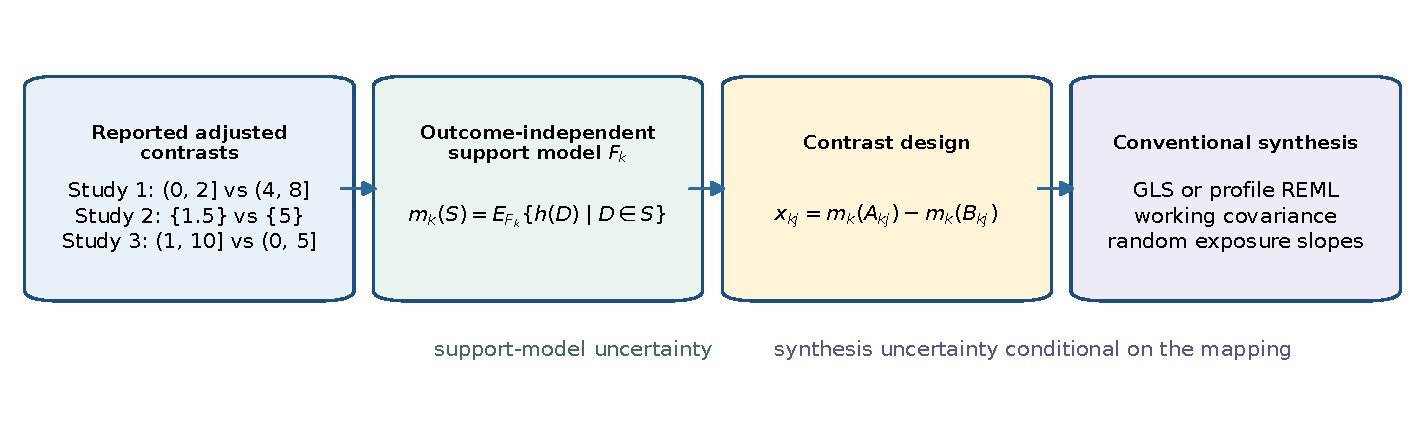
\includegraphics[width=0.98\textwidth]{images/Support_to_design_framework.pdf}
    \caption{Support-to-design framework. Each reported adjusted contrast retains its observation-specific comparison and reference supports. An outcome-independent exposure model maps each support to an average dose--response basis vector; their difference forms the contrast design passed to conventional synthesis. Support uncertainty and synthesis uncertainty are distinct.}
    \label{fig:support_design}
\end{figure}

\begin{figure}[h]
    \centering
    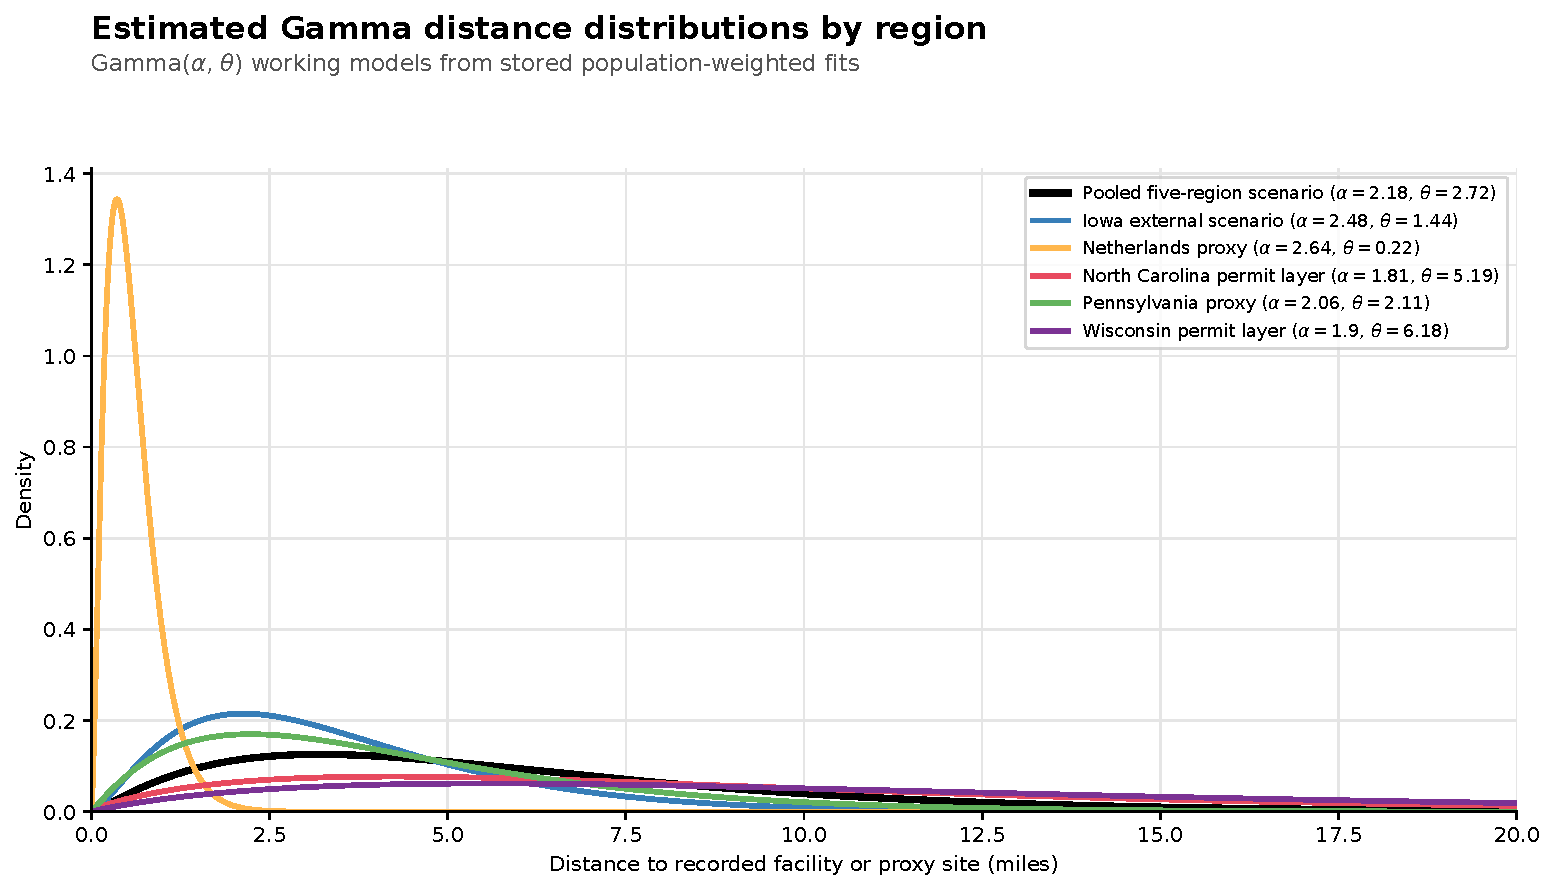
\includegraphics[width=0.96\textwidth]{images/Density_plot_Sum_Updated.pdf}
    \caption{Illustrative Gamma working distributions for residential distance to recorded facilities or proxy sites, based on population-weighted maximum likelihood. North Carolina and Wisconsin use permitted-facility layers; Pennsylvania uses an agricultural-producer directory and the Netherlands uses livestock-classified agricultural businesses in one municipality. Iowa and the displayed five-region pooled curve are external scenarios; the primary pooled sensitivities use only the four regions represented by included studies.}
    \label{fig:Residence_density}
\end{figure}

\begin{figure}[h]
    \centering
    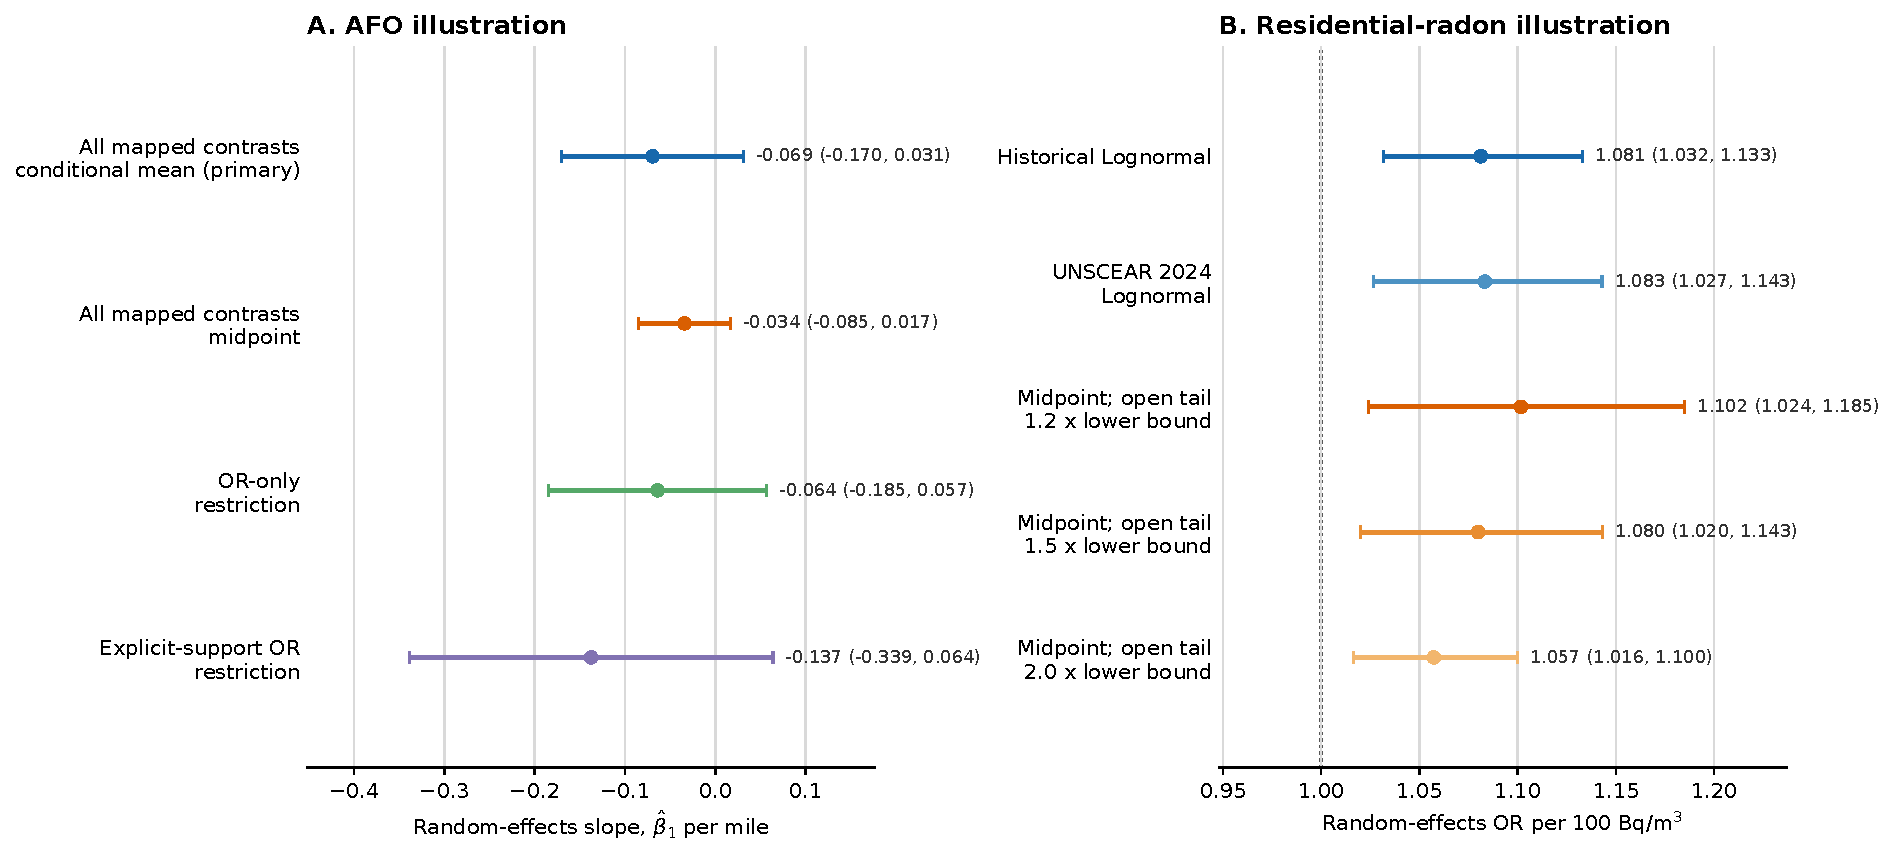
\includegraphics[width=0.96\textwidth]{images/Score_assumption_comparison.pdf}
    \caption{Direct comparison of support-representation assumptions. Panel A
    compares the primary eight-study AFO analysis under the regional Gamma
    conditional-mean and midpoint mappings, followed by the OR-only and strict
    explicit-support restrictions. Panel B compares the
    residential-radon random-effects OR per 100 Bq/m$^3$ under historical and
    current country-specific Lognormal mappings and under midpoint scoring with
    three analyst-selected rules for right-open categories. Horizontal lines are
    model-based 95\% confidence intervals; the vertical dotted line in Panel B
    marks the null OR of 1.}
    \label{fig:score_assumptions}
\end{figure}


\FloatBarrier

\section{Tables}

\begin{table}[htbp]
\centering
\caption{Primary and restriction analyses for the AFO illustration under random effects and working correlation $\rho=0.5$.}
\label{tab:real_comparison}
\small
\setlength{\tabcolsep}{3.5pt}
\begin{tabular}{llcccccc}
\toprule
Analysis & Support representation & $N$ & $K$ & $\hat\beta_1$ & SE & 95\% CI & $\hat\tau$ \\
\midrule
All mapped contrasts (primary) & Conditional mean/point & 33 & 8 & $-0.069$ & $0.051$ & $(-0.170,\ 0.031)$ & $0.129$ \\
All mapped contrasts & Midpoint/point & 33 & 8 & $-0.034$ & $0.026$ & $(-0.085,\ 0.017)$ & $0.070$ \\
OR-only restriction & Conditional mean/point & 29 & 7 & $-0.064$ & $0.062$ & $(-0.185,\ 0.057)$ & $0.146$ \\
Explicit-support OR restriction & Conditional mean/point & 15 & 4 & $-0.137$ & $0.103$ & $(-0.339,\ 0.064)$ & $0.194$ \\
\bottomrule
\end{tabular}
\par\smallskip
\begin{minipage}{0.96\textwidth}
\footnotesize $N$ is the number of contrasts and $K$ the number of independent
studies. Confidence intervals are model-based Normal intervals. The primary
study-count-$t_7$ interval was $(-0.191,0.052)$ and the
studentized parametric-bootstrap sensitivity interval was $(-0.198,0.054)$.
For the explicit-support restriction, the $t_3$ interval was
$(-0.464,0.189)$.
Restricted-likelihood values are not compared across exposure-design mappings.
\end{minipage}
\end{table}


\begin{table}[htbp]
\centering
\caption{Principal residential-radon--lung-cancer illustration from adjusted summary contrasts and external Lognormal exposure distributions.}
\label{tab:radon_example}
\small
\setlength{\tabcolsep}{4pt}
\begin{tabular}{lcccc}
\toprule
Exposure representation & $\rho$ & $\hat\beta_1$ per Bq/m$^3$ & OR per 100 Bq/m$^3$ (95\% CI) & $\hat\tau$ \\
\midrule
Historical Lognormal & $0$ & $0.001031$ & $1.109\ (1.045,\ 1.176)$ & $0.000809$ \\
Historical Lognormal & $0.25$ & $0.000872$ & $1.091\ (1.040,\ 1.145)$ & $0.000478$ \\
Historical Lognormal (primary) & $0.5$ & $0.000781$ & $1.081\ (1.032,\ 1.133)$ & $0.000468$ \\
Historical Lognormal & $0.75$ & $0.000643$ & $1.066\ (1.014,\ 1.122)$ & $0.000674$ \\
Historical Lognormal & $0.9$ & $0.000342$ & $1.035\ (0.971,\ 1.103)$ & $0.001090$ \\
UNSCEAR 2024 Lognormal & $0.5$ & $0.000800$ & $1.083\ (1.027,\ 1.143)$ & $0.000598$ \\
Midpoint; open upper $1.2a$ & $0.5$ & $0.000968$ & $1.102\ (1.024,\ 1.185)$ & $0.000887$ \\
Midpoint; open upper $1.5a$ & $0.5$ & $0.000769$ & $1.080\ (1.020,\ 1.143)$ & $0.000668$ \\
Midpoint; open upper $2.0a$ & $0.5$ & $0.000558$ & $1.057\ (1.016,\ 1.100)$ & $0.000423$ \\
\bottomrule
\end{tabular}
\par\smallskip
\begin{minipage}{0.96\textwidth}
\footnotesize The analysis contains 56 non-reference adjusted OR contrasts
from 16 studies reporting time-weighted residential radon in Bq/m$^3$. The
historical primary distributions use approximately contemporaneous national
survey parameters; UNSCEAR 2024 is a distribution-source sensitivity. In the
point-score rows, $a$ is the lower bound of a right-open support. No exposure-
group frequencies, event counts, or denominators are used. For the primary
analysis, the study-count $t$ interval for $\hat\beta_1$ was
$(0.000273,\ 0.001290)$; the CR2 sensitivity gave OR $1.081$ per 100
Bq/m$^3$ (95\% CI $1.028$--$1.137$) using the CR2 variance and a $t_{15}$
critical value, without a Satterthwaite degrees-of-freedom approximation. The studentized parametric-bootstrap
sensitivity interval was $(0.000212,\ 0.001325)$.
\end{minipage}
\end{table}


\noindent Full random-effects and fixed-effect sensitivity grids are reported in
Supplementary Tables S5 and S6.


\begin{table}[htbp]
\centering
\caption{Bias and root mean squared error (RMSE) from the mixed-support $3\times3$ profile REML simulation grid. Each setting used $R=5{,}000$ replicates.}
\label{tab:simgrid}
\begin{tabular}{cccc}
\toprule
$\beta_{1,\mathrm{true}}$ & $\tau_{\mathrm{true}}$ & Bias (RMSE), $\hat\beta_1$ & Bias (RMSE), $\hat\tau$ \\
\midrule
$-0.035$ & $0.065$ & $0.001\ (0.028)$ & $-0.006\ (0.027)$ \\
$-0.069$ & $0.065$ & $<0.001\ (0.028)$ & $-0.005\ (0.027)$ \\
$-0.139$ & $0.065$ & $>-0.001\ (0.028)$ & $-0.006\ (0.027)$ \\
$-0.035$ & $0.129$ & $>-0.001\ (0.046)$ & $-0.005\ (0.039)$ \\
$-0.069$ & $0.129$ & $<0.001\ (0.046)$ & $-0.006\ (0.039)$ \\
$-0.139$ & $0.129$ & $<0.001\ (0.047)$ & $-0.005\ (0.039)$ \\
$-0.035$ & $0.259$ & $-0.002\ (0.084)$ & $-0.008\ (0.067)$ \\
$-0.069$ & $0.259$ & $>-0.001\ (0.086)$ & $-0.009\ (0.066)$ \\
$-0.139$ & $0.259$ & $-0.001\ (0.086)$ & $-0.007\ (0.066)$ \\
\bottomrule
\end{tabular}
\par\smallskip
{\footnotesize Values smaller than $0.0005$ in magnitude are displayed as
$<0.001$ or $>-0.001$ according to direction.}
\end{table}


\begin{table}[htbp]
\centering
\caption{Point and interval performance across numbers of independent study blocks under the empirical slope and heterogeneity. Each setting used 25 resampled empirical support-and-covariance templates and $R=5{,}000$ replicates.}
\label{tab:simK}
\scriptsize
\setlength{\tabcolsep}{2.6pt}
\resizebox{\textwidth}{!}{%
\begin{tabular}{cccccccccc}
\toprule
$K$ & Bias & RMSE & Normal cov. & $t$ cov. & Normal width & $t$ width & Normal type I & $t$ type I & $\tau=0$ rate \\
\midrule
10 & $0.0001$ & $0.0451$ & $0.9150$ & $0.9482$ & $0.1710$ & $0.1974$ & $0.0832$ & $0.0526$ & $0.0020$ \\
20 & $0.0007$ & $0.0325$ & $0.9326$ & $0.9482$ & $0.1243$ & $0.1328$ & $0.0640$ & $0.0508$ & $0$ \\
30 & $-0.0007$ & $0.0263$ & $0.9356$ & $0.9482$ & $0.1021$ & $0.1065$ & $0.0556$ & $0.0470$ & $0$ \\
\bottomrule
\end{tabular}}
\par\smallskip
{\footnotesize The data-generating values were $\beta_{1,\mathrm{true}}=-0.069$ and $\tau_{\mathrm{true}}=0.129$. Type-I error was evaluated in separate null-slope cells at the same $K$ and $\tau$. Monte Carlo standard errors for coverage and type-I error were at most $0.0040$; all fits converged. The identical $0.9482$ entries at $K=10$, 20, and 30 were reproduced from simulations with distinct fixed seeds.}
\end{table}

\begin{table}[htbp]
\centering
\caption{Selected exposure-distribution and nonlinear stress tests at $K=10$ and $R=5{,}000$.}
\label{tab:simstress}
\small
\setlength{\tabcolsep}{3.5pt}
\begin{tabular}{lcccccc}
\toprule
Scenario & $\hat\beta_1$ bias & RMSE & $\hat\tau$ bias & RMSE & Normal cov. & $t$ cov. \\
\midrule
Correct Gamma working model & $0.0006$ & $0.0462$ & $-0.0066$ & $0.0393$ & $0.9066$ & $0.9376$ \\
Uniform true; Gamma fitted & $-0.2898$ & $0.3994$ & $0.7283$ & $0.8000$ & $0.8232$ & $0.9038$ \\
Nonlinear logit, $c=0.05$ & $0.0242$ & $0.0516$ & $-0.0112$ & $0.0397$ & $0.8684$ & $0.9054$ \\
Nonlinear logit, $c=0.10$ & $0.0436$ & $0.0626$ & $-0.0084$ & $0.0385$ & $0.8066$ & $0.8610$ \\
\bottomrule
\end{tabular}
\par\smallskip
{\footnotesize The true slope and heterogeneity were $-0.069469$ and $0.129253$. Monte Carlo standard errors for coverage were at most $0.0056$; all fits converged. Full stress-test results and boundary rates are in the supplement.}
\end{table}


\begin{table}[htbp]
\centering
\caption{Point-estimation performance of the fixed-effect GLS estimator. Each setting used $R=5{,}000$ mixed-support replicates.}
\label{tab:simfixed}
\begin{tabular}{cccc}
\toprule
$\beta_{1,\mathrm{true}}$ & Mean $\hat\beta_1$ & Bias & RMSE \\
\midrule
$-0.005$ & $-0.005$ & $>-0.001$ & $0.004$ \\
$-0.011$ & $-0.011$ & $<0.001$ & $0.004$ \\
$-0.022$ & $-0.022$ & $<0.001$ & $0.004$ \\
\bottomrule
\end{tabular}

\vspace{2pt}
{\footnotesize Bias values smaller than $0.001$ in magnitude are displayed as
$<0.001$ or $>-0.001$ according to direction.}
\end{table}


\noindent Detailed midpoint-comparison and stress-test results are reported in
Supplementary Tables S7--S9.

\FloatBarrier

% \section{Cross referencing}

% Environments such as figure, table, equation, align can have a label
% declared via the \verb+\label{#label}+ command. For figures and table
% environments one should use the \verb+\label{}+ command inside or just
% below the \verb+\caption{}+ command.  One can then use the
% \verb+\ref{#label}+ command to cross-reference them. As an example, consider
% the label declared for Figure \ref{fig1} which is
% \verb+\label{fig1}+. To cross-reference it, use the command
% \verb+ Figure \ref{fig1}+, for which it comes up as
% ``Figure \ref{fig1}''.
% The reference citations should used as per the ``natbib'' packages. Some sample citations:  \cite{texbook,latex:companion,latex2e,knuth:1984,lesk:1977}.

% \section{Lists}

% List in \LaTeX{} can be of three types: enumerate, itemize and description.
% In each environments, new entry is added via the \verb+\item+ command.
% Enumerate creates numbered lists, itemize creates bulleted lists and
% description creates description lists.
% \begin{enumerate}[1.]
% \item First item in the number list.
% \item Second item in the number list.
% \item Third item in the number list.
% \end{enumerate}
% List in \LaTeX{} can be of three types: enumerate, itemize and description.
% In each environments, new entry is added via the \verb+\item+ command.
% \begin{itemize}
% \item First item in the bullet list.
% \item Second item in the bullet list.
% \item Third item in the bullet list.
% \end{itemize}

\begin{Backmatter}

\paragraph{Funding Statement}
Data collection for the systematic review was funded by the National Pork Board, Des Moines, IA, United States, under grant \#19-146. The funding agency had no role in the design, implementation, analysis, interpretation, review, or preparation of this manuscript. Partial financial support was also provided by the Albert C. Dehn and Lois E. Dehn Chair in Veterinary Medicine at Michigan State University.

\paragraph{Competing Interests}
The National Pork Board funded data collection for the underlying systematic
review under grant 19-146 but had no role in the design, analysis,
interpretation, review, or preparation of this methodological manuscript. The
authors declare no other competing interests.

\paragraph{Use of Artificial Intelligence Tools}
OpenAI ChatGPT and the OpenAI Codex desktop application were accessed during
manuscript development through August 16, 2026, through the interfaces
available from \url{https://openai.com/}. Model/version labels were not
consistently retained, so no specific model number is asserted. The tools
assisted with language editing, literature-search planning, code review and
generation, implementation of author-specified simulation designs, and
interpretation checks. They did not create or alter the source data and did not
determine the statistical estimand or conclusions. The authors independently
checked cited sources, executed every analysis, regenerated simulation outputs
from the versioned code, reviewed the resulting text, and take full
responsibility for the manuscript, transformations, conclusions, and code.

\paragraph{Data Availability Statement}
The analysis-ready contrast workbooks, complete second-stage application and
simulation code, validation tests, seeds, machine-readable results, and
reproducibility instructions are available at
\url{https://github.com/ChongWangStat/IntervalDRMA}; a permanent versioned
archive DOI will be inserted before submission. The radon support and outcome
data are reconstructed from the cited public reports. The AFO association
estimates come from the living systematic-review dataset and co-author-curated
materials. Public geospatial sources underlie the stored regional AFO working-
distribution parameters, but the original observation-level distance files,
fitting scripts, and fitted covariance matrices were not retained in the
archive. Consequently, the second-stage AFO analyses are reproducible from the
stored parameters, whereas the historical first-stage fits are not fully
reconstructible. North Carolina and Wisconsin use permitted-facility sources;
Pennsylvania and the Netherlands use agricultural-site proxies as documented
in Supplementary Methods S1.

\paragraph{Ethical Standards}
This study used published aggregate effect estimates and public geospatial data and involved no new collection of individual participant or animal data. Institutional ethics approval was therefore not required.

\paragraph{Author Contributions}
Conceptualization: Yangyifan Lu, Chong Wang, and Annette M. O'Connor. Methodology: Yangyifan Lu, Chong Wang, and Annette M. O'Connor. Software: Yangyifan Lu and Chong Wang. Validation: Yangyifan Lu and Chong Wang. Writing---original draft: Yangyifan Lu, Chong Wang, and Annette M. O'Connor. Writing---review and editing: all authors. All authors approved the final submitted manuscript.


% \renewcommand\bibpreamble{By default, this template uses \texttt{bibtex} and adopts the AMS referencing style. However, the journal you’re submitting to may require a different reference style; specify the journal you're using with the class' \texttt{journal} option --- see lines 1--19 of \emph{sample.tex} for a list of options and instructions for selecting the journal.}

% If using any of the following journal options:
%   wet, dap, dce, eds, prm, flw, jdm, psy, rsm
% then use the \printbibliography line instead of:
%\bibliography{refereces}
\printbibliography

\end{Backmatter}

\end{document}
